\documentclass{itkmitlproject}

\usepackage{afterpage}
\usepackage{graphicx,amsmath,latexsym,amssymb,amsthm}
\usepackage{indentfirst}
\usepackage{cite}
\usepackage{placeins}
\usepackage[super,square]{natbib}
\usepackage{booktabs}

\setmainfont{Angsana}[
 Path = fonts/,
 UprightFont = Angsana,
 ItalicFont = *-Italic,
 BoldFont = *-Bold,
 BoldItalicFont = *-BoldItalic,
    Extension = .ttf,
    WordSpace = 0.9,
    Scale = 1.6
]

\graphicspath{ {images/} }

\makeatletter
% \patchcmd{<cmd>}{<search>}{<replace>}{<succes>}{<failure>}
\patchcmd{\@chapter}{\addtocontents{lof}{\protect\addvspace{10\p@}}}{}{}{}% LoF
\patchcmd{\@chapter}{\addtocontents{lot}{\protect\addvspace{10\p@}}}{}{}{}% LoT
\def\bibindent{2.1em}
\let\old@biblabel\@biblabel
\def\@biblabel#1{\old@biblabel{#1}\kern\bibindent}
\let\old@bibitem\bibitem
\def\bibitem#1{\old@bibitem{#1}\leavevmode\kern-\bibindent}
\makeatother

%1. Your thesis title (THAI)
\newcommand{\ThesisTitle}{ฟังก์ชันสูญเสียสำหรับการเรียนรู้ข้อมูลที่ไม่สมดุล}
%2. Your thesis title (ENG)
\newcommand{\ThesisTitleENG}{Hybrid Loss for Learning Imbalanced Data}
%3. Author name
\newcommand{\Author}{ธนวัฒน์ หลอดแก้ว}
%4. Author name ENG
\newcommand{\AuthorENG}{Thanawat Lodkaew}
%5. Author student ID
\newcommand{\SId}{59070071}
%9. Advisor name
\newcommand{\Advisor}{รองศาสตราจารย์ ดร. กิติ์สุชาต  พสุภา}
%10. Advisor name ENG
\newcommand{\AdvisorENG}{Assoc. Prof. Dr. Kitsucart  Pasupa}
%11. ภาคเรียนที่
\newcommand{\Sem}{1}
%12. ปีการศึกษา พ.ศ.
\newcommand{\AcaY}{2562}
%13. ปีการศึกษา ค.ศ.
\newcommand{\AcaYAD}{2019}
%14. วันส่งรายงาน
\newcommand{\SubD}{10 พฤศจิกายน พ.ศ. 2561}

\begin{document}    
    \frontmatter
    \lhead{}\rhead{}\chead{}\lfoot{}\cfoot{\thepage}\rfoot{}
    \makecover    
    \makeinnercover
    \makeengcover
    \makecopyrightcover
    \makethesiscert
    \makeprojectcert
   
    % Setting margin for page numbering on frontmatter
    \newgeometry{top=1in, bottom=1in, left=1.5in, right=1in, includefoot}
    
    \makeabstract{
        ปัญหาความไม่สมดุลของข้อมูล (Class Imbalance Problem) เป็นเรื่องที่ถูกหยิบขึ้นมาวิจัยอย่างแพร่หลาย เนื่องข้อมูลส่วนใหญ่มีจำนวนตัวอย่างของแต่ละกลุ่มข้อมูลไม่เท่ากัน
        ในงานวิจัยชิ้นนี้มุ่งเน้นไปที่การสร้างสรรค์แบบจำลองการเรียนรู้เชิงลึกแบบผสม (Hybrid Deep Learning) ซึ่งเป็นการผสมผสานกันระหว่างแบบจำลองการเรียนรู้เชิงลึก (Deep Learning) หลายตัว 
        มาเพื่อแก้ปัญหาดังกล่าว เนื่องจากแบบจำลอง Hybrid Deep Learning สามารถเพิ่มประสิทธิภาพในการจัดกลุ่มข้อมูลที่มีความสมดุลกันได้ ในทางเดียวกันแบบจำลองดังกล่าวอาจจะสามารถจัดกลุ่มข้อมูลที่ไม่สมดุลกันได้อย่างมีประสิทธิภาพเช่นเดียวกัน 
        ในเบื้องต้นเราได้สร้างแบบจำลอง Deep Learning แบบง่าย แล้วเพ่ิมความซับซ้อนของแบบจำลองขึ้นเรื่อย ๆ เพื่อที่จะได้แบบจำลองที่สมบูรณ์ที่สุด
    }

    \makeabstracteng{
        Classification of imbalanced data is extremely common in practice, and this problem has been widely studied in classical machine learning. 
        A classifier produced from an imbalanced data set is likely to be biased towards the majority class and show inferior classification accuracy on the minority class. 
        This work aims at inventing a hybrid deep learning model for classification on imbalanced data. Recently, many hybrid deep learning model 
        can boost the accuracy on classificaiton of balanced data. In the same way, it may work on imbalanced data effectively. Initially, a simple deep learning model is built and tested. 
        We will find out its disvantages or problems such as overfitting and then solve those by building more complex model. 
        The process will be repeated until we get a perfect model with its satisfying results.
    }

    \makeack

    \newpage
    \addcontentsline{toc}{chapter}{สารบัญ}
    \tableofcontents
    
    \newpage
    \addcontentsline{toc}{chapter}{สารบัญตาราง}
    \listoftables    
    
    \newpage
    \addcontentsline{toc}{chapter}{สารบัญภาพ}
    \listoffigures
    
    % Reset frontmatter page numbering margin, back to original margin from class file
    \restoregeometry

    \mainmatter
    \lhead{}\rhead{\thepage}\chead{}\lfoot{}\cfoot{}\rfoot{}
    
    \chapter{บทนำ}
\label{chapter:introduction}

\section{ที่มาและความสำคัญ}
ในด้านการเรียนรู้ของเครื่องจักร (Machine Learning) ความไม่สมดุลกันของข้อมูล หมายถึง การที่จำนวนตัวอย่างของแต่ละกลุ่มข้อมูลมีจำนวนไม่เท่ากัน 
ซึ่งความไม่สมดุลกันของข้อมูลนี้ถูกนิยามให้เป็นปัญหาในการจัดกลุ่มข้อมูล (Classification) สาเหตุที่ความไม่สมดุลกันของข้อมูลเป็นปัญหา คือ อัลกอริทึมการจัดกลุ่ม 
(Classification Algorithm) จะทำงานได้อย่างมีประสิทธิภาพก็ต่อเมื่อจำนวนตัวอย่างของแต่ละกลุ่มข้อมูลมีจำนวนที่เท่าหรือใกล้เคียงกัน 
เมื่อมีความไม่สมดุลกันของข้อมูลจะทำให้การทำงานของอัลกอริทึมมีประสิทธิภาพด้อยลง ซึ่งอาจจะด้อยลงจนไม่สามารถจัดกลุ่มข้อมูลได้เลย

การจัดกลุ่มข้อมูลที่มีจำนวนตัวอย่างของแต่ละกลุ่มไม่สมดุลกันเป็นเรื่องธรรมดาอย่างมากในทางปฏิบัติ 
เนื่องจากข้อมูลที่เกิดขึ้นล้วนแต่ไม่สามารถคาดเดาได้อย่างแน่นอนว่าจำนวนตัวอย่างของแต่ละกลุ่มจะสมดุลกัน อีกทั้งข้อมูลส่วนใหญ่ยังมีลักษณะที่มีจำนวนตัวอย่างของแต่ละกลุ่มไม่สมดุลกัน 
เช่น ในระหว่างวัวอยู่ในช่วงเป็นสัด ช่วงเวลาที่วัวแสดงพฤติกรรมเป็นสัดจะมีจำนวนน้อยกว่าช่วงเวลาที่วัวไม่แสดงพฤติกรรมเป็นสัด เป็นต้น ในด้านการเรียนรู้ของเครื่องจักร 
มีความเป็นไปได้ว่าตัวจัดกลุ่มข้อมูลที่ถูกสร้างขึ้นจากชุดข้อมูลที่มีจำนวนตัวอย่างของแต่ละกลุ่มไม่สมดุลกันจะมีความลำเอียงในการจัดกลุ่ม กล่าวคือ 
มีโอกาสสูงที่ตัวจัดกลุ่มจะระบุว่าข้อมูลเป็นกลุ่มส่วนมาก (Majority Class) มากกว่าเป็นกลุ่มส่วนน้อย (Minority Class) 
ซึ่งเป็นผลทำให้การระบุข้อมูลเป็นกลุ่มส่วนน้อยมีความแม่นยำที่ต่ำกว่ามาตรฐาน ซึ่งความแม่นยำในการระบุข้อมูลเป็นแต่ละกลุ่มควรจะเท่าหรือใกล้เคียงกัน

ที่ผ่านมาได้มีการศึกษาเกี่ยวกับปัญหาการจัดกลุ่มข้อมูลในลักษณะนี้อย่างกว้างขวาง และได้แสดงให้เห็นถึงความสำคัญของปัญหาของการจัดกลุ่มข้อมูลที่มีจำนวนตัวอย่างของแต่ละกลุ่มไม่สมดุลกัน 
ซึ่งทำให้ประสิทธิภาพการจัดกลุ่มข้อมูลมีความแม่นยำที่ต่ำ ดังนั้นปัญหานี้จำเป็นต้องถูกจัดการ \cite{Buda:2017} เพื่อที่จะแก้ปัญหาการจัดกลุ่มข้อมูลที่มีจำนวนตัวอย่างของแต่ละกลุ่มไม่สมดุลกัน 
ได้มีเทคนิคเกิดขึ้นมากมาย โดยสามารถแบ่งเทคนิคการแก้ปัญหาได้ 2 ระดับ คือ (1) ระดับข้อมูล (Data-Level) 
ที่ซึ่งเป็นการแก้ปัญหาโดยการจัดการข้อมูลก่อนที่จะถูกนำไปประมวลในกระบวนการจัดกลุ่มข้อมูล โดยการสุ่มเพิ่มจำนวนตัวอย่างข้อมูล (Over-Sampling) และการสุ่มลดจำนวนตัวอย่างข้อมูล 
(Under-Sampling) เป็นเทคนิคในการแก้ปัญหาในระดับข้อมูล เทคนิคการแก้ปัญหาในระดับนี้เป็นการแก้ปัญหาแบบเบื้องต้นที่สามารถดำเนินการได้ง่าย 
อย่างไรก็ตามการสุ่มเพิ่มจำนวนตัวอย่างข้อมูลสามารถทำให้เกิดปัญหา Overfitting ตามมาได้อย่างง่ายดาย 
ในทางเดียวกันการสุ่มลดจำนวนตัวอย่างข้อมูลอาจจะเป็นการกำจัดสารสนเทศที่เป็นประโยชน์ต่อการจัดกลุ่มข้อมูลออกไป (2) ระดับตัวจัดกลุ่ม (Classifier-Level) 
ที่ซึ่งเป็นการแก้ปัญหาโดยการจัดการอัลกอริทึมการจัดกลุ่ม โดยการทำเทรสโช (Thresholding) การเรียนรู้แบบความเสียหายที่รู้สึกได้ง่าย (Cost-Sensitive Learning) 
การจัดกลุ่มข้อมูลแบบหนึ่งกลุ่ม (One-Class Classification) และการผนวกกันของหลายเทคนิค อย่างไรก็ตามเทคนิคเหล่านี้มียังไม่สามารถแก้ปัญหาได้อย่างมีประสิทธิภาพในทุก ๆ ชุดข้อมูล 
กล่าวคือ เทคนิคสามารถให้ความแม่นยำในการจัดกลุ่มข้อมูลแต่ละกลุ่มได้อย่างน่าพอใจสำหรับชุดข้อมูล A แต่ไม่สามารถทำได้อย่างมีประสิทธิภาพสำหรับชุดข้อมูล B เป็นต้น 
ดังนั้นเทคนิคใหม่ที่จะสามารถการแก้ปัญหาการจัดกลุ่มข้อมูลที่ไม่สมดุลกันได้อย่างมีประสิทธิภาพ และปรับเข้าได้กับทุกชุดข้อมูลจำเป็นต้องถูกคิดค้นขึ้น

\section{ความมุ่งหมายและวัตถุประสงค์ของการศึกษา}
\begin{enumerate}
	\item เพื่อศึกษาการจัดการปัญหาความไม่สมดุลกันของข้อมูลด้วยเทคนิคต่าง ๆ
\end{enumerate}
\section{ขอบเขตการพัฒนาโครงงาน}
\begin{enumerate}
	\item ทดลองใช้เทคนิคการจัดกลุ่มข้อมูลที่ไม่สมดุลกันแบบต่าง ๆ ในแต่ละชุดข้อมูล เพื่อค้นหาว่าเทคนิคที่ดีที่สุด
\end{enumerate}
\section{ขั้นตอนการดำเนินงาน}
\begin{enumerate}
	\item ศึกษาเกี่ยวกับนิยามของความไม่สมดุลกันของข้อมูลในด้านการจัดกลุ่มข้อมูล
	\item ศึกษารูปแบบการแก้ปัญหาการจัดกลุ่มข้อมูลที่ไม่สมดุลกันแบบต่าง ๆ
	\item ศึกษางานวิจัยที่เกี่ยวข้อง
	\item ตั้งข้อสมมติฐาน
	\item ออกแบบการทดลอง
	\item เลือกชุดข้อมูล และ Metrics ที่จะใช้ในการทดลอง
	\item ดำเนินการทำการทดลอง
	\item สรุปผลการทดลอง
\end{enumerate}
\section{ประโยชน์ที่คาดว่าจะได้รับ}
\begin{enumerate}
	\item เทคนิคในการสร้างแบบจำลองการจัดกลุ่มข้อมูลที่สามารถให้ความแม่นยำที่สูงในการระบุข้อมูลแต่กลุ่ม แม้ว่าแบบจำลองจะเรียนรู้จากชุดข้อมูลที่ไม่สมดุลกัน
\end{enumerate}


    \chapter{การทบทวนวรรณกรรมที่เกี่ยวข้อง}
\label{chapter:literature-review}

\section{ทฤษฎีที่เกี่ยวข้อง}
\subsection{ปัญหาความไม่สมดุลกันของกลุ่มข้อมูล}
ความไม่สมดุลกันของกลุ่มข้อมูล คือ การที่ตัวอย่างของข้อมูลแต่ละกลุ่มมีจำนวนไม่เท่ากัน และจำนวนตัวอย่างนั้นต่างกันมาก เช่น ชุดข้อมูล A มี 2 กลุ่มข้อมูลจากทั้งหมด 10,500 ตัวอย่าง 
แบ่งออกเป็นกลุ่มข้อมูลที่ 1 จำนวน 500 ตัวอย่าง และกลุ่มข้อมูลที่ 2 จำนวน 10,000 เป็นต้น 

ในงานวิจัย~\cite{Anand:1993} ผู้วิจัยได้ทำการศึกษาเกี่ยวกับผลทระทบของความไม่สมดุลกันของข้อมูลในการเรียนรู้ของโมเดล และพบว่าความไม่สมดุลกันของข้อมูลได้ส่งผลกระทบด้านลบต่อกระบวนการ Backpropagation โดยผลกระทบดังกล่าว คือ การที่กลุ่มข้อมูลส่วนมากมีอิทธิพลต่อค่า Gredient ที่จะถูกนำไปใช้ในการปรับค่า Weight มากกว่ากลุ่มข้อมูลส่วนน้อย เนื่องจากจำนวนตัวอย่างของกลุ่มข้อมูลส่วนมากในแต่ละ Batch ของการเรียนรู้ นั้นมีมากกว่า ทำให้ค่าสูญเสียรวมมีลักษณะที่ค่าสูญของกลุ่มข้อมูลส่วนมากไปกลบค่าสูญเสียของกลุ่มข้อมูลส่วนน้อย 

เหตุการณ์ดังกล่าวทำให้ลักษณะของการเรียนรู้ของโมเดลมุ่งไปที่การเรียนรู้เฉพาะกลุ่มข้อมูลส่วนมาก  กล่าวคือ ค่าสูญเสียของกลุ่มข้อมูลส่วนมากจะลดลงอย่างรวดเร็ว ในขณะที่ค่าสูญเสียของกลุ่มข้อมูลส่วนน้อยเพิ่มขึ้นเรื่อย ๆ ในช่วงต้นของการเรียนรู้ สุดท้ายทำให้การเรียนรู้ของโมเดลเข้าลู่เข้าจุดที่ดีที่สุดช้าหรือไม่สามารถเรียนรู้ที่จะจัดกลุ่มได้เลย

ความไม่สมดุลกันของกลุ่มข้อมูลนั้นมีอยู่ 2 ประเภท คือ Step Imbalance~\cite{Buda:2017} และ Long-Tailed Imbalance~\cite{Liu:2019} ตามรายละเอียดดังนี้

\begin{itemize}
  \item Step Imbalance เป็นความไม่สมดุลกันของกลุ่มข้อมูลที่จำนวนตัวอย่างของกลุ่มข้อมูลส่วนน้อยแต่ละกลุ่มมีจำนวนเท่ากัน และจำนวนตัวอย่างของกลุ่มข้อมูลส่วนมากแต่ละกลุ่มมีจำนวนเท่ากัน โดยอัตราส่วนของกลุ่มของส่วนน้อยและส่วนมาก ($\mu$) สามารถคำนวณได้จากสมการที่ \ref{eq:stepimbalance} ตัวอย่างการกระจายของจำนวนตัวอย่างของกลุ่มข้อมูลแสดงดังรูปที่ \ref{fig:imb-dist:1} และ \ref{fig:imb-dist:2} 
  \begin{equation}
      \mu = \frac{\left | \left \{ i\in  \left \{ 1,...,N \right \}: C_{i}\:is\:minority\:class \right \} \right |}{N},
      \label{eq:stepimbalance}
    \end{equation}

    โดยที่ $C_{i}$ คือ ชุดของตัวอย่างของกลุ่มข้อมูล $i$ และ N คือ จำนวนกลุ่มตัวอย่างทั้งหมด
  \item Long-Tailed Imbalance เป็นความไม่สมดุลกันของกลุ่มข้อมูลที่จำนวนตัวอย่างของแต่ละกลุ่มข้อมูลมีจำนวนไม่เท่ากันตามตัวอย่างการกระจายของจำนวนตัวอย่างของกลุ่มข้อมูลในรูปที่ \ref{fig:imb-dist:3}
  
\end{itemize}

สามารถคำนวณค่าอัตราส่วนระหว่างจำนวนตัวอย่างของกลุ่มข้อมูลส่วนน้อยและกลุ่มข้อมูลส่วนมาก ($p$) สำหรับวามไม่สมดุลกันของกลุ่มข้อมูลทั้งสองประเภทได้ตามสมการที่ \ref{eq:p_ratio}

\begin{equation}
  p = \frac{max_{i}\left \{ \left | C_{i} \right | \right \}}{min_{i}\left \{ \left | C_{i} \right | \right \}}
  \label{eq:p_ratio}
\end{equation}

\begin{figure}[h]
  \centering
  \subfigure[]{
      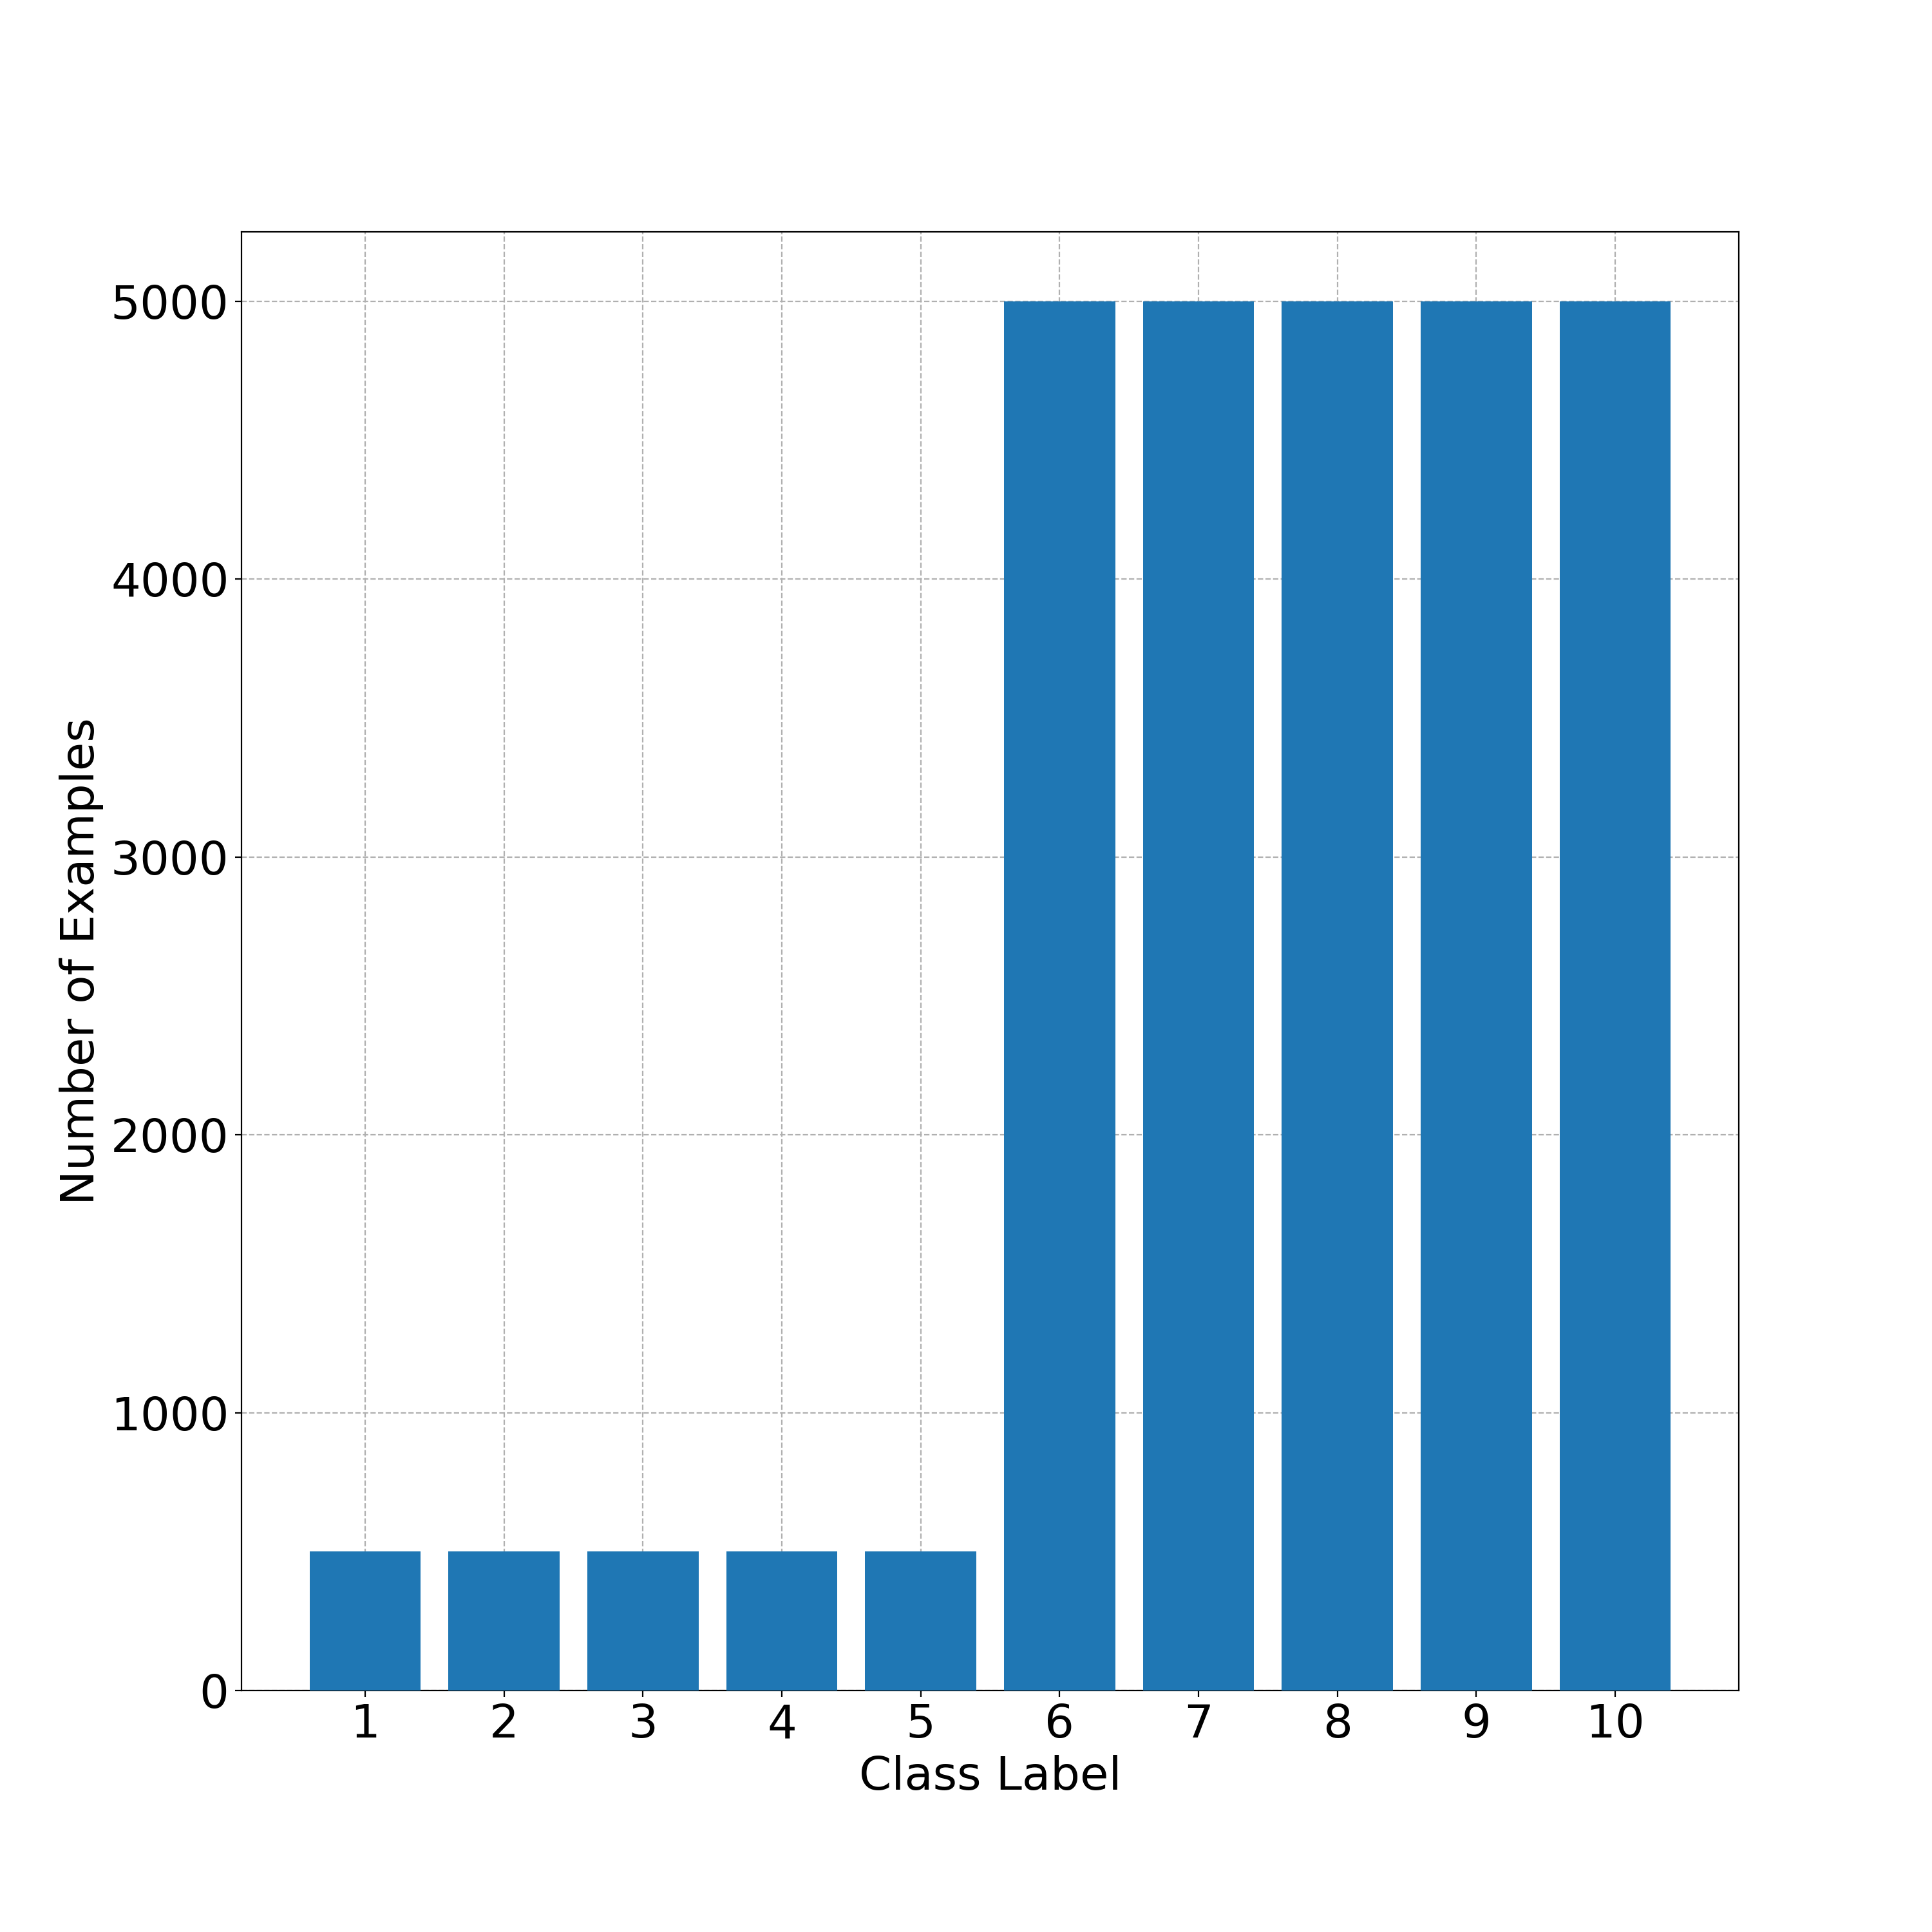
\includegraphics[width=0.45\columnwidth]{imbalance-distribution-1}
      \label{fig:imb-dist:1}
  }
  \subfigure[]{
      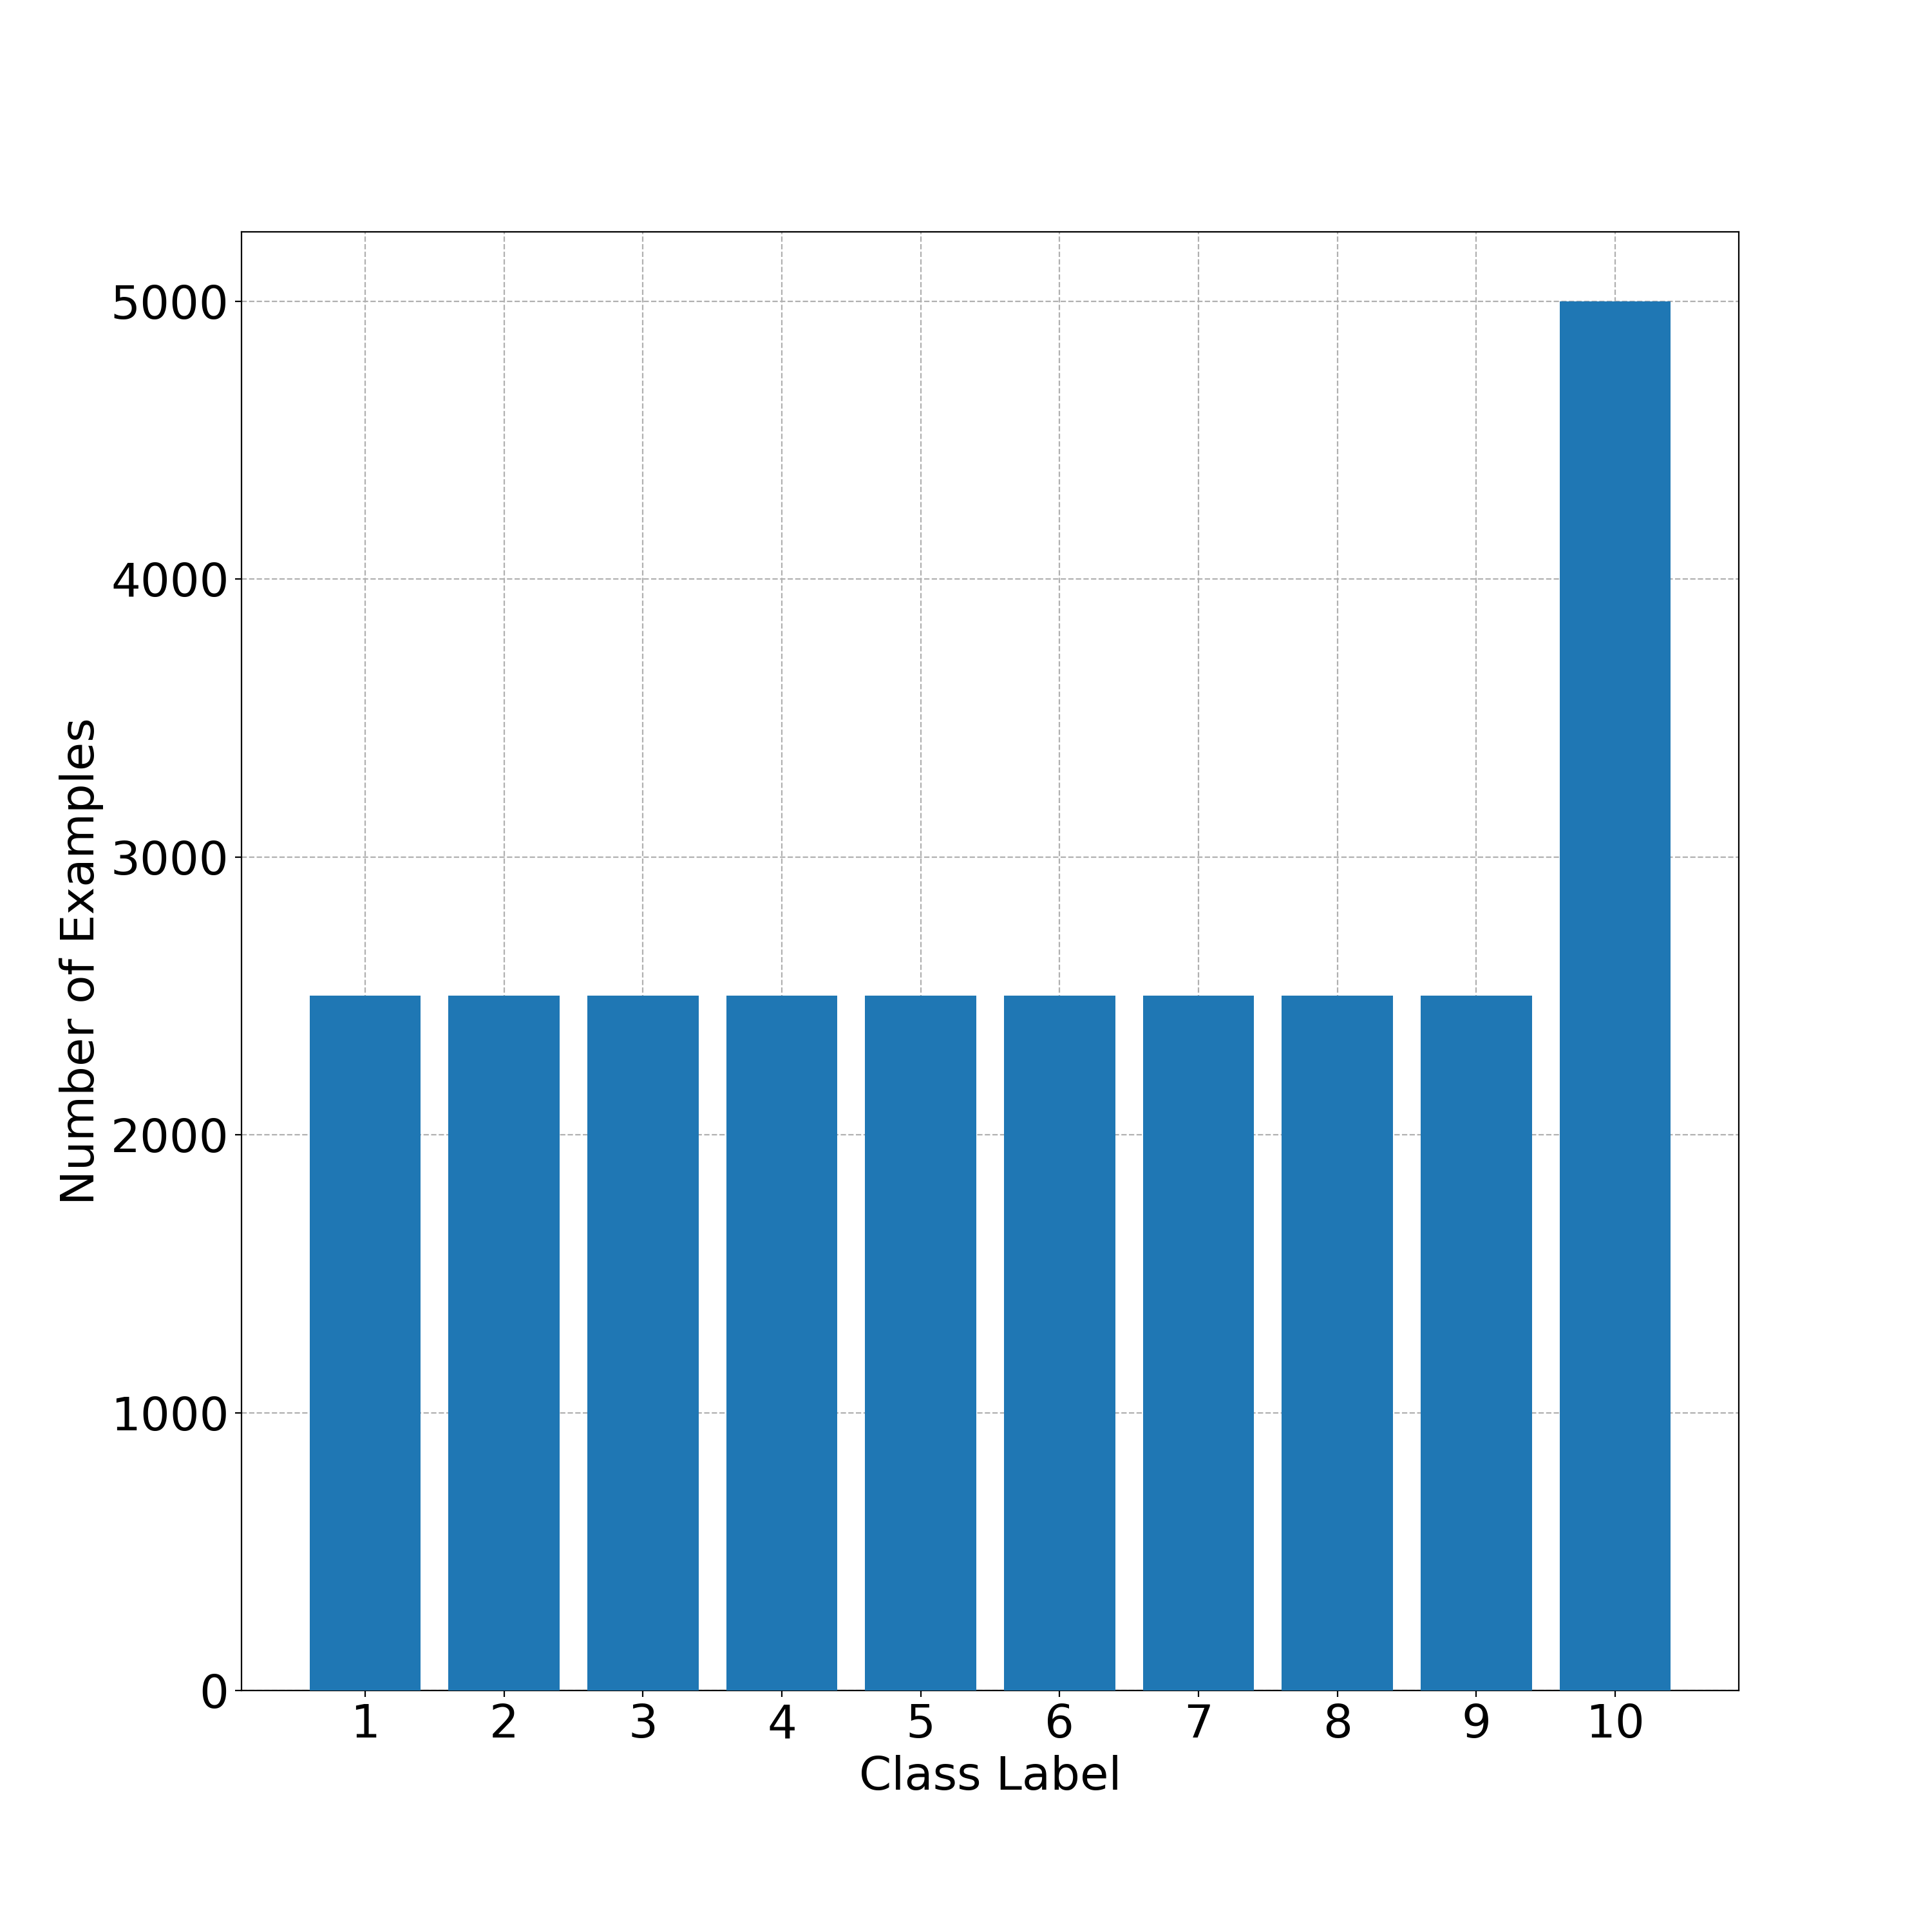
\includegraphics[width=0.45\columnwidth]{imbalance-distribution-2}
      \label{fig:imb-dist:2}
  }
  \subfigure[]{
    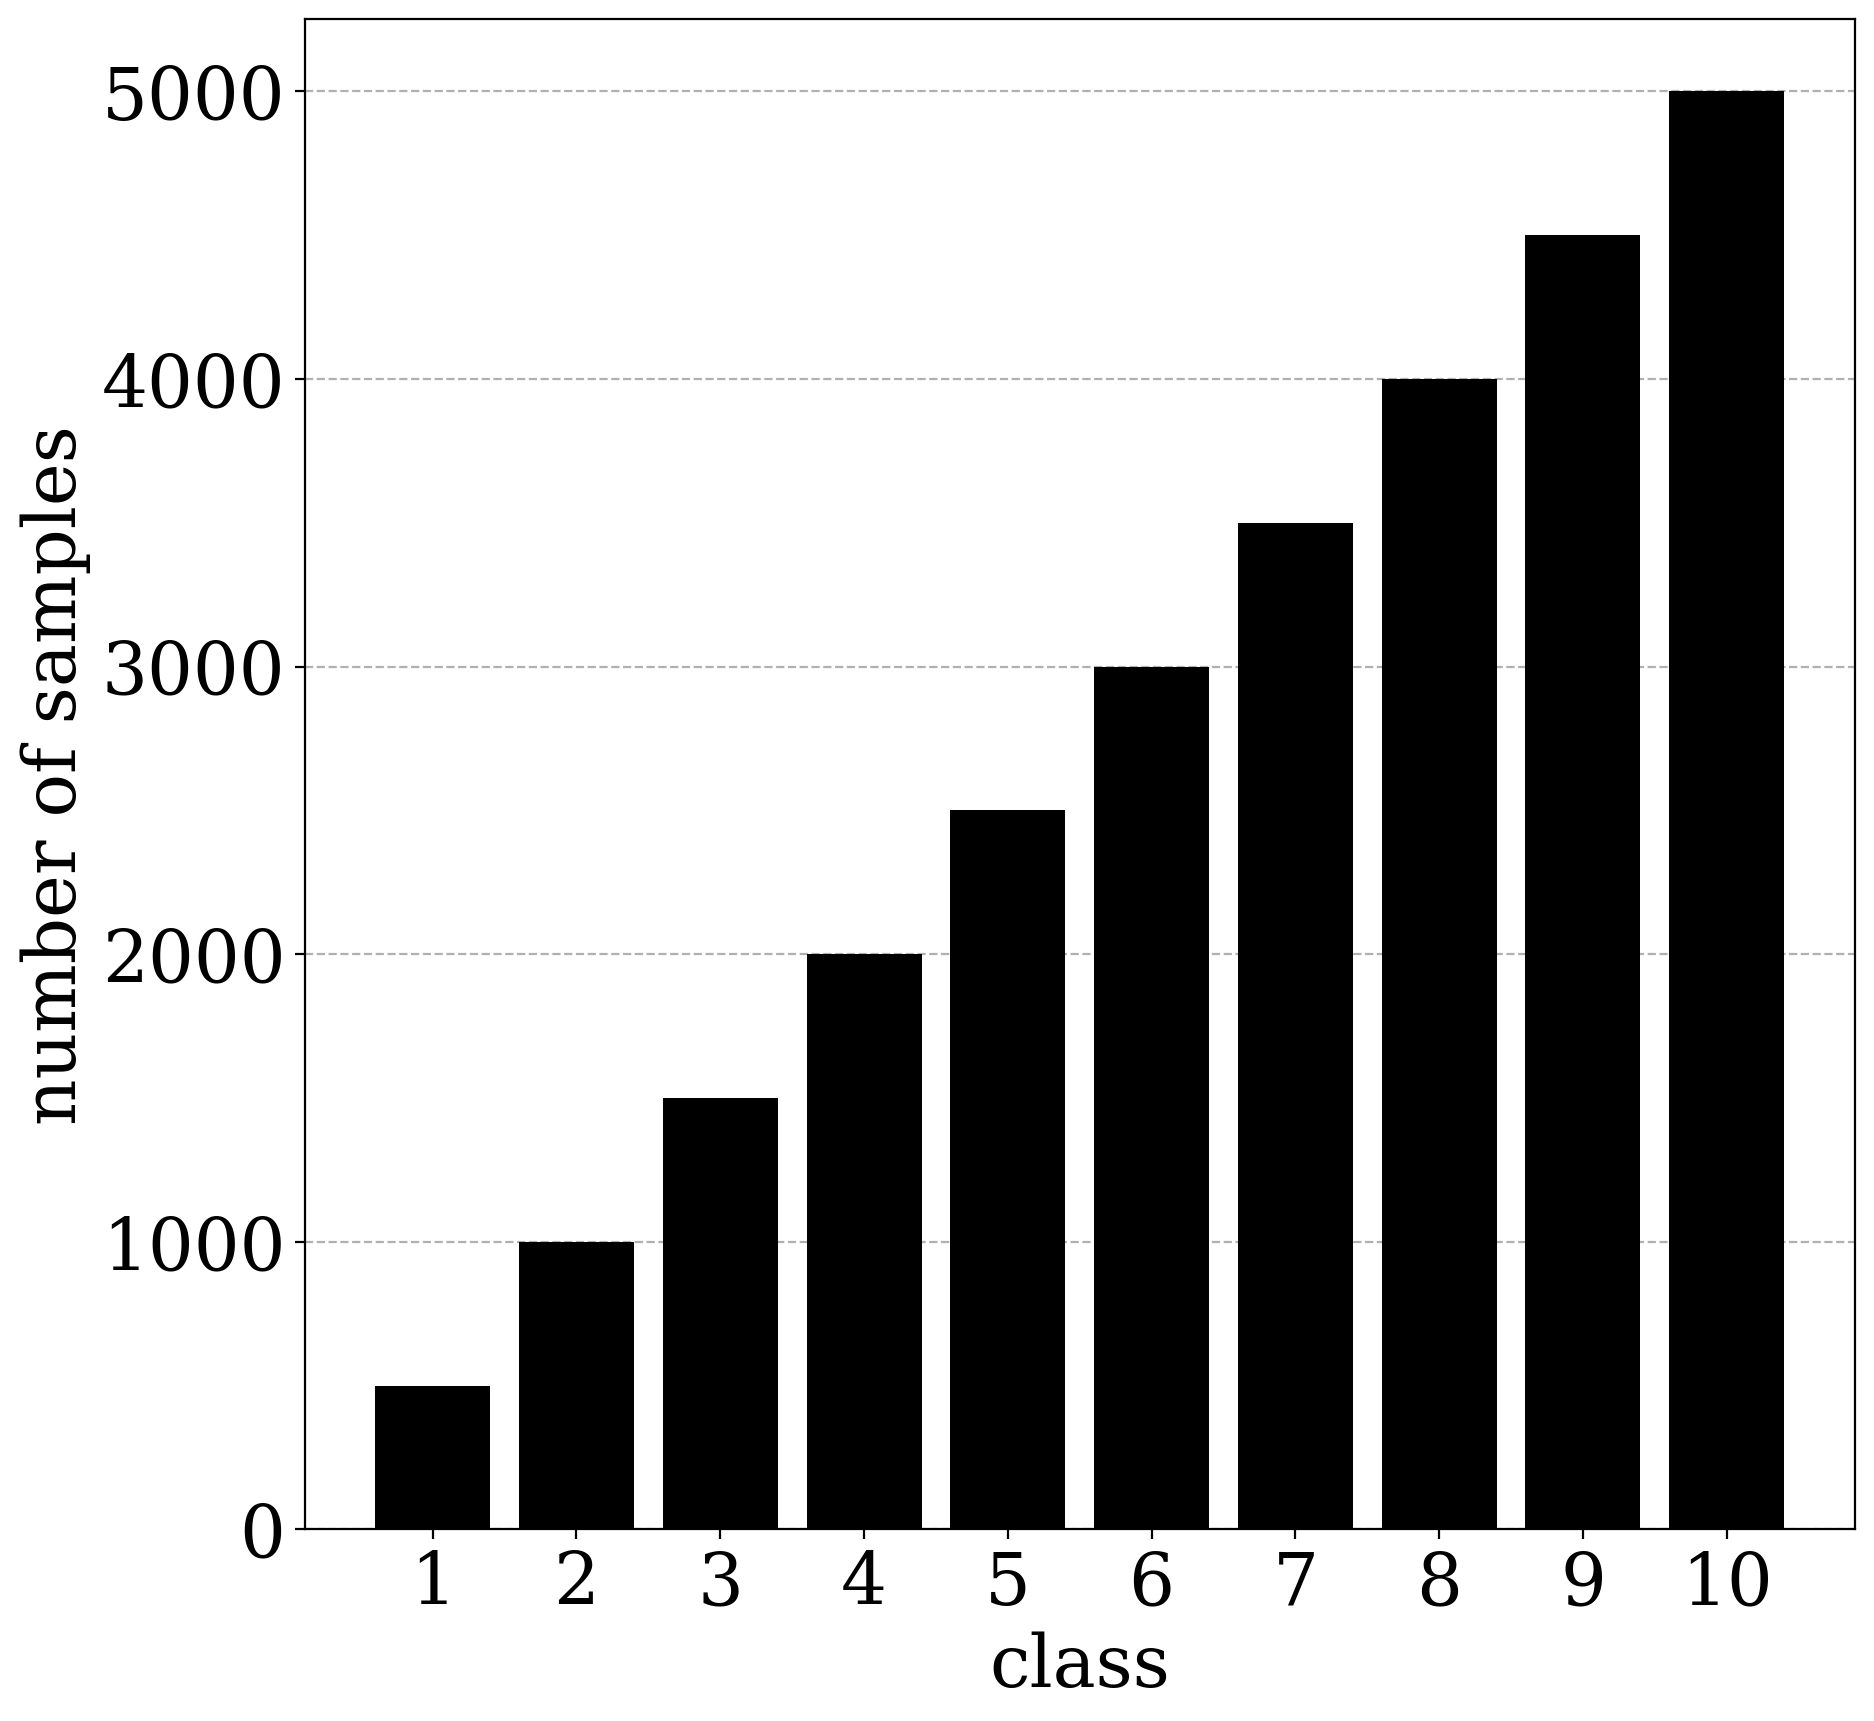
\includegraphics[width=0.45\columnwidth]{imbalance-distribution-3}
    \label{fig:imb-dist:3}
  }
  \caption{ตัวอย่างการกระจายของจำนวนตัวอย่างของกลุ่มข้อมูล (ก) $p = 10$, $\mu = 0.5$ (ข) $p = 2$, $\mu = 0.9$ (ค) $p = 10$}
  \label{fig:imb-dist}
\end{figure}
\FloatBarrier

\subsection{การจัดการปัญหาความไม่สมดุลกันของกลุ่มข้อมูลด้วยวิธีการต่าง ๆ}
\subsubsection{Cost-Sensitive Learning}
Cost-Sensitive Learning เป็นหนึ่งในเทคนิคการเรียนรู้ของอัลกอริทึมการจัดกลุ่มข้อมูลที่มีการนำ ค่าความเสียหายของการระบุกลุ่มข้อมูลผิดพลาด (Misclassification Cost) มาพิจารณาเพื่อที่จะพยายามลดค่าความเสียหายดังกล่าวให้น้อยที่สุด~\cite{Ling-CS:2010} 
ในกระบวนการเรียนรู้ของอัลกอริทึมการจัดกลุ่มข้อมูล ส่วนใหญ่พยายามที่จะลดอัตราความผิดพลาดในการระบุกลุ่มข้อมูลให้น้อยที่สุด ซึ่งอัตราความผิดพลาด คือ อัตราของการระบุกลุ่มข้อมูลผิด 
โดยแบ่งออกเป็นสองประเภท คือ ความผิดพลาดที่ระบุข้อมูลกลุ่ม Positive เป็นกลุ่ม Negative (False Negative) และ ความผิดพลาดที่ระบุข้อมูลกลุ่ม Negative เป็นกลุ่ม Positive (False Positive) 
อัลกอริทึมดังกล่าวจะพยายามลดความผิดพลาดโดยรวม กล่าวคือ ให้ความสำคัญที่ False Negative และ False Positive เท่ากัน

ในความเป็นจริงบางครั้งความผิดพลาดดังกล่าวไม่ควรให้ความสำคัญเท่ากัน เช่น ในการตรวจวินิฉัยโรคมะเร็ง ที่ซึ่งผู้ป่วยที่มีโรคมะเร็งเป็นข้อมูลกลุ่ม Positive และผู้ป่วยที่มีสุขภาพดีเป็นข้อมูลกลุ่ม Negative 
การวินิจฉัยผิดพลาดว่าผู้ป่วยมีสุขภาพดี แต่จริง ๆ แล้วมีโรคมะเร็ง (False Negative) นั้นมีความเสียหายมากกว่าการที่วินิจฉัยผิดพลาดว่าผู้ป่วยมีโรคมะเร็ง แต่จริง ๆ แล้วมีสุขภาพดี (False Positive) ดังนั้นควรจะให้ความสำคัญที่ False Negative มากกว่า เป็นต้น 

Cost-Sensitive Learning จะให้ความสำคัญกับความเสียหายดังกล่าวไม่เท่ากัน ที่ซึ่ง False Negative จะถูกให้ความสำคัญมากกว่า และเรียกว่าเป็นค่าความเสียหายของการระบุกลุ่มข้อมูลผิดพลาด ค่าความเสียหายถูกระบุไว้ดังตารางที่ \ref{table:2:cost-matrix} ซึ่งเรียกว่า Cost Matrix โดยที่ C(i,j) คือ ค่าความเสียหายในการระบุข้อมูลกลุ่ม j เป็นกลุ่ม i

โดยปกติแล้ว Cost-Sensitive ถูกนำมาใช้ในการแก้ปัญหาความไม่สมดุลกันของข้อมูล เนื่องจาก โดยทั่วไปกลุ่มข้อมูลส่วนใหญ่นั้นจะเป็นกลุ่ม Positive และข้อมูลกลุ่ม Positive มักจะถูกระบุผิดว่าเป็นกลุ่ม Negative

\begin{table}[]
	\caption{ตัวอย่างของ Cost Matrix สำหรับการจัดกลุ่มข้อมูลสองกลุ่ม โดย 1 คือ Positive และ 0 คือ Negative}
	\label{table:2:cost-matrix}
	\centering
  \begin{tabular}{l|l|l|}
    \cline{2-3}
     & \textbf{Actual Negative} & \textbf{Actual Positive} \\ \hline
    \multicolumn{1}{|l|}{Predict Negative} & C(0,0), or TP & C(0,1), or \emph{FN} \\ \hline
    \multicolumn{1}{|l|}{Predict Positive} & C(1,0), or \emph{FP} & C(1,1), or TP \\ \hline
    \end{tabular}
\end{table}
\FloatBarrier

\subsection{การเรียนรู้เชิงลึก (Deep Learning)}
Ian Goodfellow et al. \cite{Goodfellow:2016} ได้อธิบายว่า การเรียนรู้เชิงลึกเป็นวิธีการที่สามารถแก้ปัญหาที่ดำเนินการได้ง่ายสำหรับมนุษย์ แต่ยากต่อการอธิบาย 
กล่าวคือ ปัญหาเหล่านั้นเป็นปัญหาที่เราสามารถแก้ได้อย่างอัตโนมัตด้วยสัญชาตญาณ  เช่น การจดจำคำพูด หรือใบหน้าผู้คนในรูป เป็นต้น 
สามารถเรียกปัญหาหรืองานประเภทนี้ว่า งานที่เป็นรูปแบบ (Formal Task) ในทางตรงกันข้าม ปัญหาหรืองานที่ไม่เป็นรูปแบบ (Informal Task) 
ที่ซึ่งยากสำหรับมนุษย์ในการดำเนินการ แต่ง่ายสำหรับการประมวลของคอมพิวเตอร์ ปัญหาประเภทนี้จะสามารถถูกอธิบายออกมาในรูปแบบของสมการคณิตศาสตร์ 
หรือมีวิธีการคำนวณทางคณิตศาสตร์ได้ เช่น การพยากรณ์สภาพอากาศ ที่ซึ่งปัจจัยต่าง ๆ ที่เกี่ยวข้อง อย่าง ค่าความชื้น ค่าอุณหภูมิวันก่อนหน้า และค่าอื่น ๆ 
จะถูกนำมาคำนวณ เป็นต้น

การเรียนรู้เชิงลึกทำให้คอมพิวเตอร์สามารถเรียนรู้จากประสบการณ์ และเข้าใจสิ่งต่าง ๆ แบบเป็นลำดับชั้นของแนวคิดเหมือนกับมนุษย์ 
โดยที่แต่ละลำดับชั้นของแนวคิดถูกกำหนดผ่านความสัมพันธ์กับชั้นของแนวคิดที่ไม่ซับซ้อน กล่าวคือ 
แนวคิดที่เป็นลำดับชั้นทำให้คอมพิวเตอร์สามารถเรียนรู้แนวคิดที่ซับซ้อนโดยการสร้างมันจากแนวคิดที่ไม่ซับซ้อน 

ในศาสตร์ทางด้านปัญญาประดิษฐ์ (Artificial Intelligence: AI) การที่ระบบคอมพิวเตอร์สามารถได้รับมาซึ่งความรู้จากการสกัดรูปแบบของข้อมูลดิบ 
เรียกความสามารถนี้ว่า การเรียนรู้ของเครื่องจักร อัลกอริธึมพื้นฐานของการเรียนรู้ของเครื่องจักรอย่าง Logistic Regression 
Linear Regression หรือ Naive Bayes สามารถประมวลเพื่อดำเนินงานที่เป็นรูปแบบต่าง ๆ เช่น พยากรณ์สภาพอากาศ 
แนะนำช่วงเวลาสำหรับการคลอดลูก หรือแยกแยะอีเมลที่ถูกต้องออกจากอีเมลขยะ เป็นต้น ประสิทธิภาพของอัลกอริธึมพื้นฐานเหล่านั้นขึ้นอยู่กับคุณลักษณะ (Feature) ของข้อมูลที่ได้รับ ตัวอย่างเช่น เมื่อการถดถอยโลจิสติกส์ถูกใช้ในการพยากรณ์โรคมะเร็งเต้านม หมอจะต้องให้ข้อมูลที่เกี่ยวข้องแก่อัลกอริธึม 
เช่น เต้านมมีผื่น แดง ร้อน ผื่นคล้ายผิวส้มหรือไม่ และมีก้อนหนาๆ ในเต้านมหรือใต้แขนหรือไม่ เป็นต้น ข้อมูลดังกล่าวเป็นคุณลักษณะของคนไข้ 
ซึ่งเรียกแต่ละประเภทข้อมูลว่า คุณลักษณะ การถดถอยโลจิสติกส์จะเรียนรู้ว่าคุณลักษณะเหล่านั้นมีความสัมพันธ์กันอย่างไรกับผลลัพธ์ ซึ่งผลลัพธ์ในตัวอย่างนี่คือ 
โอกาสในการเป็นโรคมะเร็งเต้านม อย่างไรก็ตามอัลกอริธึมไม่สามารถกำหนดได้ว่าคุณลักษณะต้องถูกกำหนดมาอย่างไร กล่าวคือ 
การได้มาซึ่งค่าของคุณลักษณะไม่ใช่หน้าที่ของอัลกอริทึม เพราะฉะนั้นถ้าอัลกอริธึมได้รับภาพ MRI มาเพื่อพยากรณ์โรคมะเร็งเต้านม แทนการใช้ข้อมูลที่เป็นรูปแบบของหมอ 
จะทำอัลกอริธีมไม่สามารถพยากรณ์ผลลัพธ์ที่เป็นประโยชน์ได้ หรือผลลัพธ์ที่ได้จะไม่น่าเชื่อถือเลย เพราะค่า Pixel ในภาพ MRI 
ไม่ได้มีความสัมพันธ์กันกับลักษณะความผิดปกติของเต้านมอย่างสิ้นเชิง

แบบจำลองพื้นฐานของการเรียนรู้เชิงลึก คือ Multi-Layer Perceptron (MLP) ที่ซึ่งเป็นเพียงฟังก์ชันคณิตศาสตร์ที่ทำการแปลงค่าข้อมูลขาเข้าไปเป็นข้อมูลขาออก ฟังก์ชันจะถูกสร้างขึ้นจากการประกอบเข้าด้วยกันของหลายฟังก์ชันที่เป็นพื้นฐานกว่า 
เราสามารถใช้ฟังก์ชันที่ต่างกันในแต่ละงานเพื่อให้ได้มาซึ่งคุณลักษณะของข้อมูลที่เหมาะสมกับงานนั้น ๆ

\subsubsection{การเรียนรู้ของโมเดล Deep Learning}

\section{งานวิจัยที่เกี่ยวข้อง}
เมื่อเทคนิคการจัดกลุ่มข้อมูลที่ประกอบด้วยโครงข่ายประสาทแบบคอนโวลูชันถูกใช้กับชุดข้อมูลที่มีความไม่สมดุลกัน อัตราการพยากรณ์ผิดพลาดจะมีค่าสูงเมื่อเทียบกับการเพิ่มขึ้นของจำนวนรอบของการเรียนรู้ของแบบจำลอง กล่าวคือ ยิ่งจำนวนรอบของการเรียนรู้สูงขึ้น จะทำให้อัตราการพยากรณ์ผิดพลาดสูงขึ้นด้วย \cite{Yan:2015} เบื้องหลังของสาเหตุที่ทำให้เป็นเช่นนั้น คือ ในเสตจของการเรียนรู้ของแบบจำลองการเรียนรู้เชิงลึก ข้อมูลจะถูกแบ่งออกเป็นกลุ่ม ๆ ซึ่งทำให้แต่ละกลุ่มมีความไม่เท่าเทียมกันเมื่อข้อมูลไม่สมดุลกัน อีกทั้งบางกลุ่มอาจจะมีแค่ตัวอย่างของกลุ่มข้อมูลที่เป็นส่วนมาก หรือกลุ่มข้อมูลที่เป็นส่วนน้อยเท่านั้น เมื่อแบบจำลองได้เรียนรู้ข้อมูลจากกลุ่มเหล่านั้นในทุก ๆ รอบ จึงทำให้เกิดอัตราการพยากรณ์ผิดพลาดที่สูง

เมื่อไม่นานมานี้ได้มีงานวิจัยที่พยายามจัดการกับปัญหาการเรียนรู้ของแบบจำลองการเรียนรู้เชิงลึกเมื่อต้องเรียนรู้ข้อมูลที่มีความไม่สมดุลกัน ดังต่อไปนี้
    \chapter{วิธีการดำเนินการวิจัย}
\label{chapter:experiment}

\section{Hybrid Loss}
\subsection{Focal Loss}
สิ่งดลใจในการคิดค้น Focal Loss (FL)~\cite{Lin:2017} คือ Cross Entropy ไม่สามารถควบคุมความสมดุลระหว่างค่าสูญเสียจากกลุ่มข้อมูลส่วนมากและค่าสูญเสียจากกลุ่มข้อมูลส่วนน้อยได้ เพราะข้อมูลจากทั้งสองกลุ่มไม่สมดุลกัน แม้ว่าการใส่ Weighting Factor ($\alpha$) จะสามารถแก้ปัญหานี้ได้ในเบื้องต้น แต่มันก็ไม่สามารถที่จะแยกความแตกต่างระหว่าง ตัวอย่างที่ง่าย (ตัวอย่างที่ให้ค่าสูญเสียน้อย) และ ตัวอย่างที่ยาก (ตัวอย่างที่ให้ค่าสูญเสียมาก) ได้ ซึ่งตัวอย่างที่ง่ายของกลุ่มข้อมูลส่วนมากจะส่วนในการคำนวณค่าสูญเสียรวมมาก ทำให้มีอิทธิพลต่อการคำนวณค่า Gradient มากเช่นเดียวกัน ซึ่งโดยปกติแล้วตัวอย่างที่ยากของกลุ่มข้อมูลส่วนมากจะประกอบไปด้วยข้อมูลที่เป็นประโยชน์ต่อการจัดกลุ่มมากกว่าตัวอย่างที่ง่ายของ
กลุ่มข้อมูลส่วนน้อย~\cite{Zhu:2019} ดังนั้นการเรียนรู้จากตัวอย่างที่ยากของกลุ่มข้อมูลส่วนมากจะมีประสิทธิภาพมากกว่าการเรียนรู้จากตัวอย่างที่ง่ายของกลุ่มข้อมูลส่วนมาก

จากที่กล่าวมาข้างต้นทำให้มีความจำเป็นที่จะต้องลดการมีส่วนร่วมในการคำนวณค่าสูยเสียรวมของตัวอย่างที่ง่าย และให้ความสนใจที่การมีส่วนร่วมในการคำนวณค่าสูยเสียรวมของตัวอย่างที่ยาก ดังนั้น FL ถูกออกแบบมาเพื่อการนี้โดยการเพิ่ม Modulating Factor ($(1 - p_{t})^{\gamma}$) เข้าไปใน Cross Entropy เพื่อที่จะลดน้ำหนักของการเรียนรู้จากตัวอย่างที่ง่าย ที่ซึ่ง Modulating Factor จะช่วยลดการมีส่วนร่วมในการคำนวณค่าสูญเสียรวมจากตัวอย่างที่ง่ายและมุ่งไปที่การเรียนรู้จากตัวอย่างที่ยาก สำหรับการคำนวณค่าสูญเสียและค่าสูญเสียรวมของ FL สามารถคำนวณได้ตามสมการที่~\ref{eq:fl} และ~\ref{eq:tfl} ตามลำดับ

\begin{equation} \label{eq:fl}
FL(p_{t}) = - \alpha_{i}(1 - p_{t})^\gamma \log (p_{t})
\end{equation}

\begin{equation} \label{eq:tfl}
    l_{FL} = \frac{1}{n} \sum_{i = 1}^{n} -\alpha_{i}(1 - p_{t}^{i})^{\gamma}\log (p_{t}^{i})
\end{equation}

สมการด้านบนเป็น FL ในรูปแบบที่เพิ่ม Weighting Factor เข้ามาด้วยเพื่อควบคุมความสมดุลระหว่างค่าสูญเสียจากกลุ่มข้อมูลส่วนมากและค่าสูญเสียจากกลุ่มข้อมูลส่วนน้อย โดยที่ $\gamma$ คือ Focusing Parameter และสำหรับค่าของ $p_{t}$ สามารถถูกระบุได้ดังสมการที่~\ref{eq:p}

\begin{equation} \label{eq:p}
	p_{t} = 
	\begin{cases}
		p & \text{ if } y = 1\\ 
		1 - p & \text{ otherwise, } 
	\end{cases}
\end{equation} 

โดยที่ $p$ คือ ค่าความน่าจะเป็นในการทำนายของโมเดล ดังนั้น $p_{t}^{i}$ คือ ค่า $p_{t}$ ของตัวอย่าง $i$

ในทางปฎิบัติ $\alpha_{i}$ จะมีค่าเท่ากับ $\alpha$ ถ้ากลุ่มข้อมูลของตัวอย่าง $i$ คือ กลุ่มข้อมูลส่วนน้อย และจะมีค่าเท่ากับ $1-\alpha$ ถ้ากลุ่มข้อมูลของตัวอย่าง $i$ คือ กลุ่มข้อมูลส่วนมาก

\subsection{Mean False Error}
Mean False Error (MFE)~\cite{Wang:2016} เป็นฟังก์ชันสูญเสียที่ถูกแก้ไขมาจาก Mean Squared Error (MSE) สิ่งจูงใจในการคิดค้นฟังก์ชันสูญเสียนี้ขึ้นมา คือ MSE ไม่สามารถตรวจจับค่าสูญเสียจากกลุ่มข้อมูลส่วนน้อยได้อย่างมีประสิทธิภาพ พูดง่าย ๆ คือ ค่าสูญเสียรวมที่คำนวณด้วย MSE มันจะมาจากค่าเฉลี่ยของค่าสูญเสียของข้อมูลทั้งหมด โดยสมการคำนวณค่าสูญเสียของ MSE และ สมการคำนวณค่าสูญเสียรวม แสดงดังสมการที่~\ref{eq:mse} และ~\ref{eq:tmse} ตามลำดับ

\begin{equation} \label{eq:mse}
    MSE = \frac{1}{2}(y - d)^{2}
\end{equation}

\begin{equation} \label{eq:tmse}
    l_{MSE} = \frac{1}{n}\sum_{i=1}^{n}\frac{1}{2}(y^{i} - d^{i})^{2}
\end{equation}

จากสมการด้านบน $l$ คือ ค่าสูญเสียรวม, $n$ คือ จำนวนตัวอย่างทั้งหมด, $y^{i}$ ค่ากลุ่มข้อมูลจริงของตัวอย่าง $i$ และ $d^{i}$ คือ ค่าทำนายของโมเดลของตัวอย่าง $i$ โดยที่ $d$ สามารถคำนวณได้จากฟังก์ชัน Logistic ใด ๆ เช่น ฟังก์ชัน Sigmoid ดังสมการที่~\ref{eq:sigmoid} เป็นต้น

\begin{equation} \label{eq:sigmoid}
d =  \frac{\mathrm{1} }{\mathrm{1} + e^{-x} }
\end{equation}

โดยที่ $x$ คือ เอ๊าต์พุตจาก Layer ก่อนหน้า

จากคำนวณค่าสูญเสียรวมด้วย MSE นั้นหมายความว่าค่าสูญเสียจากกลุ่มข้อมูลส่วนมากจะไปกลบค่าสูญเสียจากกลุ่มข้อมูลส่วนน้อย เนื่องจากจำนวนตัวอย่างของกลุ่มข้อมูลส่วนมากนั้นมีมากกว่า เพื่อที่จะแก้ปัญหานี้ MFE ถูกออกแบบให้สามารถคำนวณค่าสูญเสียรวมด้วยการรวมกันระหว่าง ค่าสูญเสียเฉลี่ยของกลุ่มข้อมูลส่วนน้อย กับ ค่าสูญเสียเฉลี่ยของกลุ่มข้อมูลส่วนมาก ตามสมการที่~\ref{eq:mfe} ซึ่ง

\begin{equation} \label{eq:mfe}
    l_{MFE} = \frac{1}{n\_major}\sum_{i=1}^{n\_major}\frac{1}{2}(y^{i} - d^{i})^{2} +\frac{1}{n\_minor}\sum_{i=1}^{n\_minor}\frac{1}{2}(y^{i} - d^{i})^{2}
\end{equation}

โดยที่ $n\_major$ คือ จำนวนตัวอย่างของกลุ่มข้อมูลส่วนมาก และ $n\_minor$ คือ จำนวนตัวอย่างของกลุ่มข้อมูลส่วนน้อย

ผลการทดลองใช้ MFE ในการเรียนรู้ของโมเดลกับชุดข้อมูล CIFAR-100 แสดงให้เห็นว่า MFE สามารถให้ผลการทำนายที่แม่นยำมากกว่า MSE อย่างสิ้นเชิง~\cite{Wang:2016}

\subsection{นิยามของ Hybrid Loss}
คุณสมบัติที่สำคัญของ FL คือ มันสามารถควบความแตกต่างระหว่างตัวอย่างที่ง่ายและตัวอย่างที่ยาก ยิ่งไปกว่านั้นการที่เพิ่ม $\alpha$ เข้าไปในการคำนวณค่าสูญเสียยังช่วยทำให้ความสำคัญของตัวอย่างของกลุ่มข้อมูลส่วนน้อยและส่วนมากมีความสมดุลกัน อย่างไรก็ตามในเมื่อค่าสูญเสียรวมคือค่าเฉลี่ยของค่าสูญเสียของข้อมูลทั้งหมด มันก็ยังมีโอกาสที่ค่าสูญเสียจากกลุ่มข้อมูลส่วนมากจะไปกลบค่าสูญเสียจากกลุ่มข้อมูลส่วนน้อย ถ้าเราแก้ปัญหาด้วยการกำหนดค่า $\alpha$ ให้มีค่าที่มาก ก็อาจจะช่วยแก้ปัญหานี้ได้ในเบื้องต้น ผลการทดลองใน~\cite{Lin:2017} ได้แสดงให้เห็นว่าการที่ $\alpha$ มีค่าที่มากก็ไม่ทำให้ประสทธิภาพของโมเดลดีไปกว่าค่าที่น้อยกว่าเลย ดังนั้นการเพิ่ม $\alpha$ เข้าไปในการคำนวณค่าสูญเสียอาจจะไม่เพียงพอในการแก้ปัญหานี้

เพื่อที่จะควบคุมค่าสูญเสียจากกลุ่มข้อมูลส่วนมากและกลุ่มข้อมูลส่วนน้อยให้มีความสมดุลกันอย่างสิ้นเชิง
ในงานวิจัยนี้จึงได้เสนอที่จะนำรูปแบบการคำนวณค่าสูญเสียรวมของ MFE มาประยุกต์ใช้ร่วมกับการคำนวณค่าสูญเสียของ FL กล่าวคือ การคำนวณค่าสูญเสียของแต่ละตัวอย่างยังคงเหมือนเดิมตามการคำนวณด้วย FL แต่ในการคำนวณค่าสูญเสียรวมจะเป็นการนำค่าสูญเสียเฉลี่ยของกลุ่มข้อมูลส่วนมากและค่าสูญเสียเฉลี่ยของกลุ่มข้อมูลส่วนน้อยมาบวกกัน ดังสมการที่~\ref{eq:hybird1}

\begin{equation} \label{eq:hybird1}
    l_{Hybrid} = \frac{1}{n\_major} \sum_{i = 1}^{n\_major} -\alpha_{i}(1 - p_{t}^{i})^{\gamma}\log (p_{t}^{i}) + \frac{1}{n\_minor} \sum_{i = 1}^{n\_minor} -\alpha_{i}(1 - p_{t}^{i})^{\gamma}\log (p_{t}^{i})
\end{equation}

\subsection{การหาอนุพันธ์}

\subsubsection{อนุพันธ์ของ FL}
กำหนดให้มี $x$ และ $y$ โดยที่ $y$ คือ ค่ากลุ่มข้อมูลจริง สมมติให้

\begin{equation}
	p = \sigma (x) = \frac{1}{1 + e^{-x}}
\end{equation}

ดังนั้น

\begin{equation}
	p_{t} = \frac{1}{1 + e^{xy}}
\end{equation}

เมื่อหาอนุพันธ์ของ $p_{t}$ เทียบกับ $x$ จะได้

\begin{equation}
\frac{dp_{t}}{dx} = y(1 - p_{t})p_{t}
\end{equation}

กำหนดให้

\begin{equation}
    l_{FL} = \frac{1}{n} \sum_{i = 1}^{n} - (1 - p_{t}^{i})^{\gamma}\log (p_{t}^{i})
\end{equation}

โดยที่ $\gamma$ เป็นค่าคงที่ เมื่อหาอนุพันธ์ของ $l_{FL}$ เทียบกับ $x$จะได้

\begin{equation}
\begin{split}
\frac{dl_{FL}}{dx} & = \frac{1}{n} \sum_{i = 1}^{n} (\frac{dl_{FL}}{dp_{t}^{i}} * \frac{dp_{t}^{i}}{dx^{i}}) \\
& =\frac{1}{n} \sum_{i = 1}^{n} [\gamma (1 - p_{t}^{i})^{\gamma - 1} \log (p_{t}^{i}) + \frac{(1 - p_{t}^{i})^{\gamma}}{p_{t}^{i}}] * [y^{i}(1 - p_{t}^{i})p_{t}^{i}]  \\
& = \frac{1}{n} \sum_{i = 1}^{n} y^{i} (1 - p_{t}^{i})^{\gamma} (\gamma p_{t}^{i} \log (p_{t}^{i}) + p_{t}^{i} - 1)
\end{split}
\end{equation}

\subsubsection{อนุพันธ์ของ MFE}
กำหนดให้

\begin{equation}
MSE_{major} = \frac{1}{n\_major}\sum_{i=1}^{n\_major}\frac{1}{2}(y^{i} - d^{i})^{2}
\end{equation}

\begin{equation}
MSE_{minor} = \frac{1}{n\_minor}\sum_{i=1}^{n\_minor}\frac{1}{2}(y^{i} - d^{i})^{2}
\end{equation}

ดังนั้น

\begin{equation}
    l_{MFE} = MSE_{major} + MSE_{minor}
\end{equation}

เมื่อหาอนุพันธ์ของ $l_{MFE}$ เทียบกับ $x$ จะได้

\begin{equation}
\frac{dl_{MFE}}{dx} = \frac{dMSE_{major}}{dx} + \frac{dMSE_{minor}}{dx}
\end{equation}

โดยที่

\begin{equation} \label{eq:fpe_derivative}
\frac{dMSE_{major}}{dx} = - \frac{1}{n\_major} \sum_{i=1}^{n\_major} (y^{i} - d^{i}) d^{i} (1 - d^{i})
\end{equation}

\begin{equation} \label{eq:fne_derivative}
\frac{dMSE_{minor}}{dx} = - \frac{1}{n\_minor} \sum_{i=1}^{n\_minor} (y^{i} - d^{i}) d^{i} (1 - d^{i})
\end{equation}

เราจะใช้อนุพันธ์ที่ต่างกันสำหรับตัวอย่างของแต่ละกลุ่มข้อมูล กล่าวคือ ถ้าเป็นตัวอย่างของกลุ่มข้อมูลส่วนมาก สมการที่~\ref{eq:fpe_derivative} จะถูกใช้ และสมการที่~\ref{eq:fne_derivative} จะถูกใช้เมื่อตัวย่างเป็นของกลุ่มข้อมูลส่วนน้อย



\subsubsection{อนุพันธ์ของ Hybrid Loss}
กำหนดให้

\begin{equation}
    FL_{major} = \frac{1}{n\_major} \sum_{i = 1}^{n\_major} - (1 - p_{t}^{i})^{\gamma}\log (p_{t}^{i})
\end{equation}

\begin{equation}
    FL_{minor} = \frac{1}{n\_minor} \sum_{i = 1}^{n\_minor} - (1 - p_{t}^{i})^{\gamma}\log (p_{t}^{i})
\end{equation}

ดังนั้น

\begin{equation}
    l_{Hybrid} = FL_{major} + FL_{minor}
\end{equation}

เมื่อหาอนุพันธ์ของ $l_{Hybrid}$ เทียบกับ x จะได้

\begin{equation}
\frac{dl_{Hybrid}}{dx} = \frac{dFL_{major}}{dx} + \frac{dFL_{minor}}{dx}
\end{equation}

โดยที่

\begin{equation} \label{fl_major_derivative}
\frac{dFL_{major}}{dx} = \frac{1}{n\_major} \sum_{i = 1}^{n\_major} y^{i} (1 - p_{t}^{i})^{\gamma} (\gamma p_{t}^{i} \log (p_{t}^{i}) + p_{t}^{i} - 1)
\end{equation}

\begin{equation} \label{fl_minor_derivative}
\frac{dFL_{minor}}{dx} = \frac{1}{n\_minor} \sum_{i = 1}^{n\_minor} y^{i} (1 - p_{t}^{i})^{\gamma} (\gamma p_{t}^{i} \log (p_{t}^{i}) + p_{t}^{i} - 1)
\end{equation}

เช่นเดียวกับการใช้อนุพันธ์ของ MFE ก็คือ เราจะใช้สมการที่~\ref{fl_major_derivative} ถ้าตัวอย่างเป็นของกลุ่มข้อมูลส่วนมาก และจะใช้สมการที่~\ref{fl_minor_derivative} ถ้าตัวอย่างเป็นของกลุ่มข้อมูลส่วนน้อย

\section{Metrics สำหรับการประเมินประสิทธิภาพของโมเดล}
\subsection{F1-Score}
F1-Score เป็นค่าเฉลี่ยของ Precision และ Recall ที่ซึ่งเราสามารถพิจารณาประสิทธิภาพของแบบจำลองด้วย F1-Score แทนการพิจารณาด้วย Precision หรือ Recall โดย F1-Score สามารถคำนวณได้จากสมการที่ \ref{eq:f1-score}

\begin{equation}
  F1 = 2 * \left ( \frac{precision * recall}{precision + recall} \right )
  \label{eq:f1-score}
\end{equation}

โดยที่ Precision และ Recall สามารถคำนวณได้จากสมการที่ \ref{eq:precision} และ \ref{eq:recall} ตามลำดับ

\begin{equation}
  precision = \frac{TP}{TP + FP}
  \label{eq:precision}
\end{equation}

\begin{equation}
  recall = \frac{TP}{TP + FN}
  \label{eq:recall}
\end{equation}

โดยที่

\begin{itemize}
  \item True Positive (TP) คือ จำนวนตัวอย่างที่แบบจำลองตรวจจับได้ว่าเป็น Positive Class และตัวอย่างเหล่านั้นเป็น Positive Class
  \item True Negative (TN) คือ จำนวนตัวอย่างที่แบบจำลองตรวจจับได้ว่าเป็น Negative Class และตัวอย่างเหล่านั้นเป็น Negative Class
  \item False Positive (FP) คือ จำนวนตัวอย่างที่แบบจำลองตรวจจับได้ว่าเป็น Positive Class แต่ตัวอย่างเหล่านั้นเป็น Negative Class
  \item False Negative (FN) คือ จำนวนตัวอย่างที่แบบจำลองตรวจจับได้ว่าเป็น Negative Class แต่ตัวอย่างเหล่านั้นเป็น Positive Class
\end{itemize}

\subsection{Receiver Operating Characteristic Curve (ROC Curve)}
ROC Curve เป็นกราฟความสัมพันธ์ระหว่าง True Positive Rate (TPR) และ False Positive Rate (FPR) โดย TPR หรือ Recall คือ 
ความน่าจะเป็นที่แบบจำลองสามารถตรวจจับ Positive Class จากจำนวน Positive Class ทั้งหมด และ FPR คือ 
ความน่าจะเป็นที่แบบจำลองจะตรวจจับ Positive Class จากจำนวน Negative Class ทั้งหมด ทั้ง TPR และ FPR สามารถคำนวณได้จากสมการที่ \ref{eq:tpr} และ \ref{eq:fpr} ตามลำดับ

\begin{equation}
  TPR = recall = \frac{TP}{TP + FN}
  \label{eq:tpr}
\end{equation}

\begin{equation}
  FPR = \frac{FP}{FP + TN}
  \label{eq:fpr}
\end{equation}

\subsection{Area Under the ROC Curve (AUC)}
AUC คือความน่าจะเป็นที่แบบจำลองจะระบุตัวอย่างของ Positive Class ว่าเป็น Positive Class และตัวอย่างของ Negative Class ว่าเป็น Negative Class 
โดยถ้าค่า AUC เข้าใกล้ 1 นั้นหมายความว่าแบบจำลองมีความสามารถในการแยก Positive Class ออกจาก Negative Class ได้เป็นอย่างดี 
ในทางเทคนิค AUC ก็คือพื้นที่ใต้กราฟของ ROC Curve โดยความสัมพันธ์กันระหว่างค่า AUC และ ROC Curve ถูกแสดงดังรูปที่ \ref{fig:roc}

\begin{figure}[h]
  \centering
  \subfigure[]{
      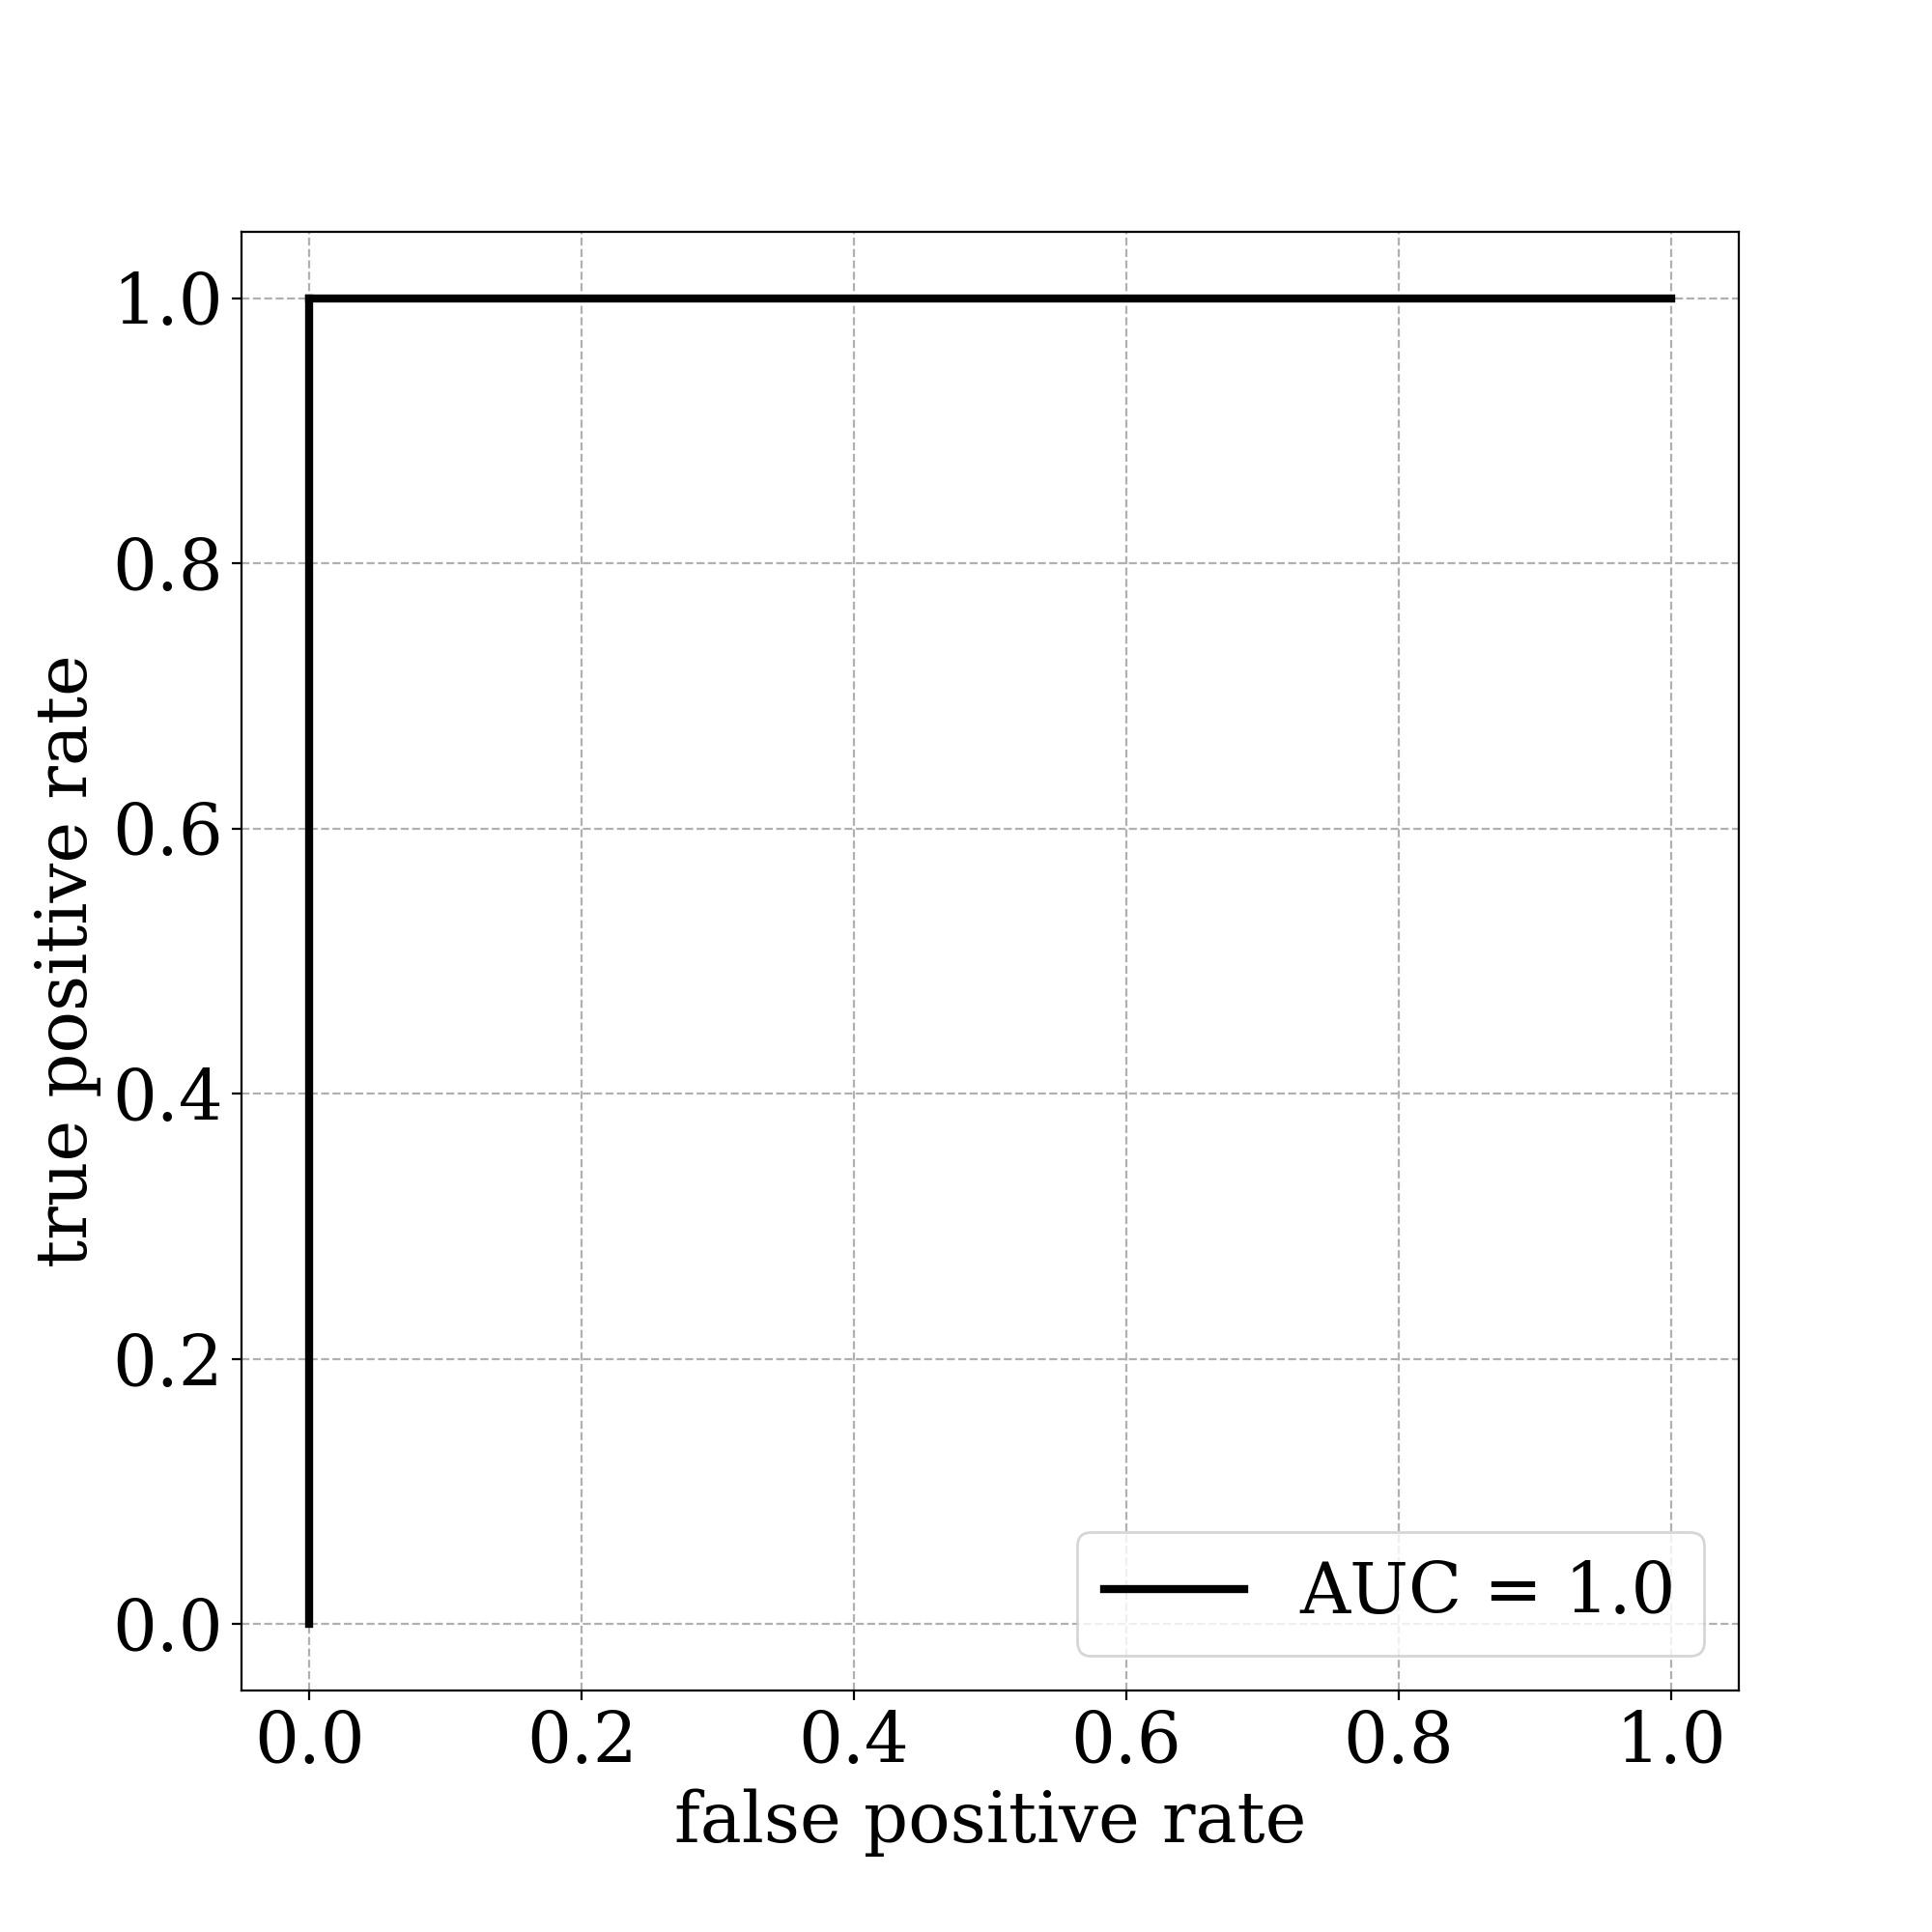
\includegraphics[width=0.45\columnwidth]{roc-1.png}
      \label{fig:roc:1}
  }
  \subfigure[]{
      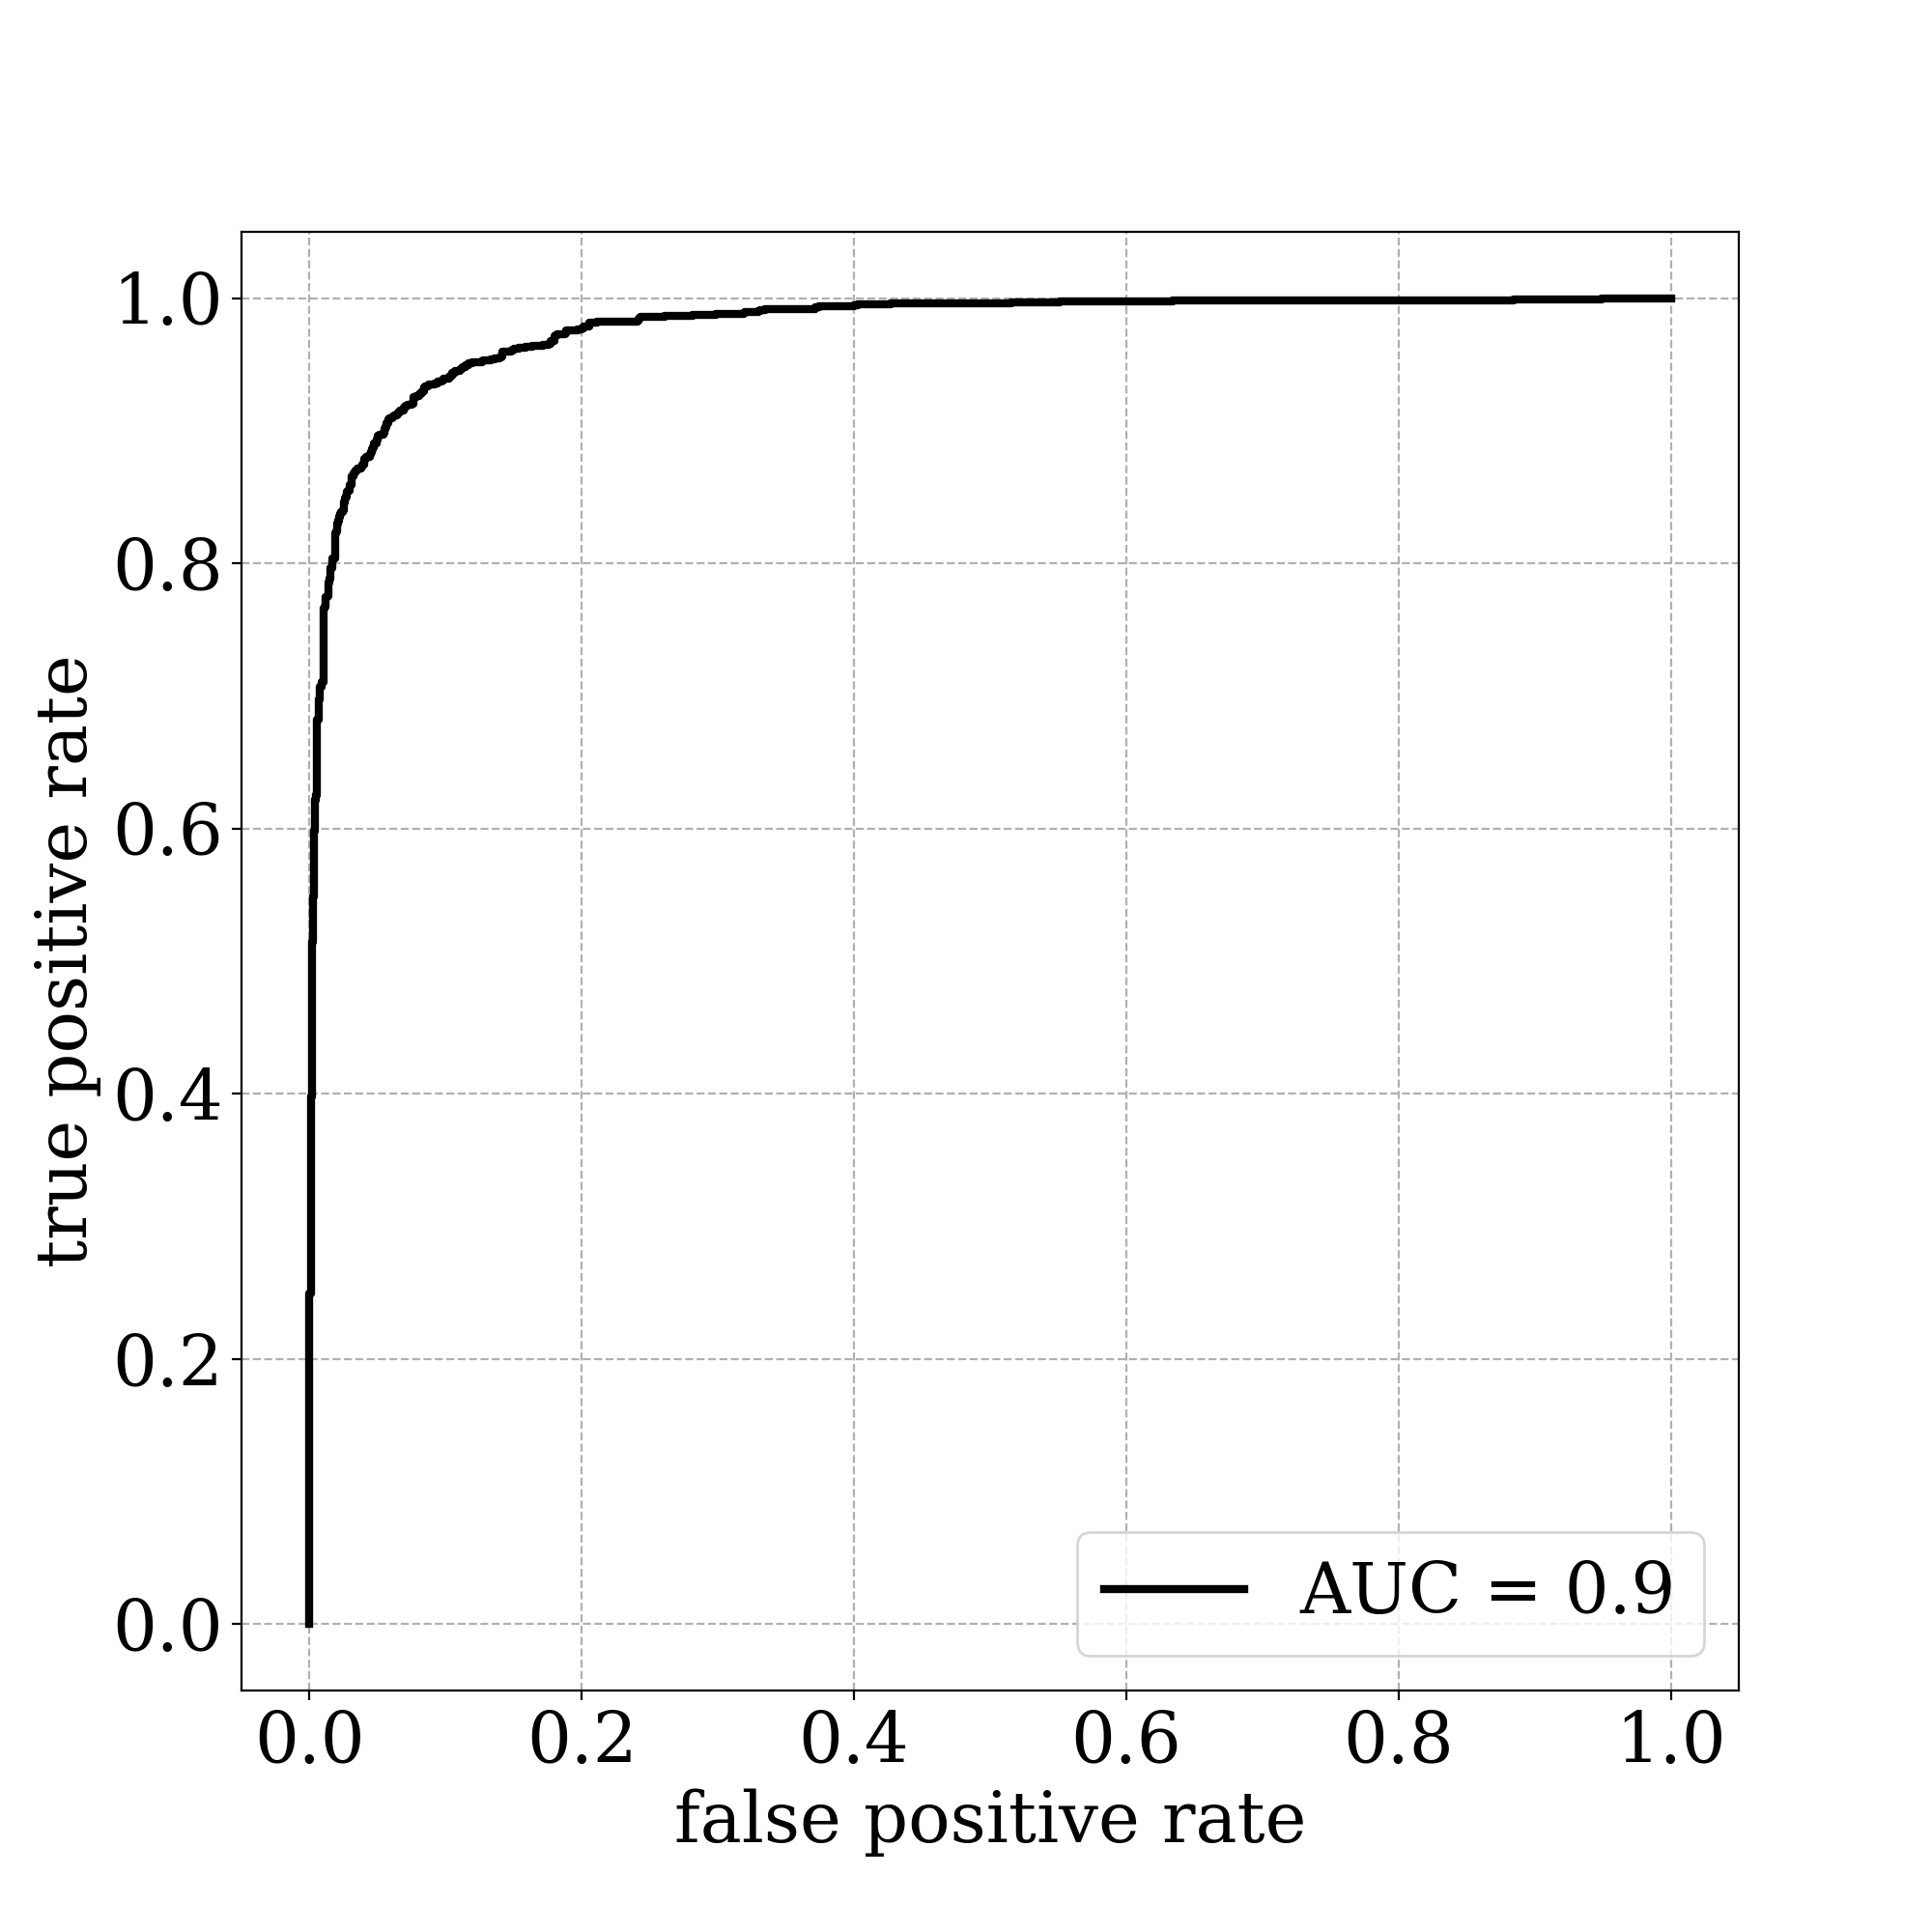
\includegraphics[width=0.45\columnwidth]{roc-2.png}
      \label{fig:roc:3}
  }
  \subfigure[]{
    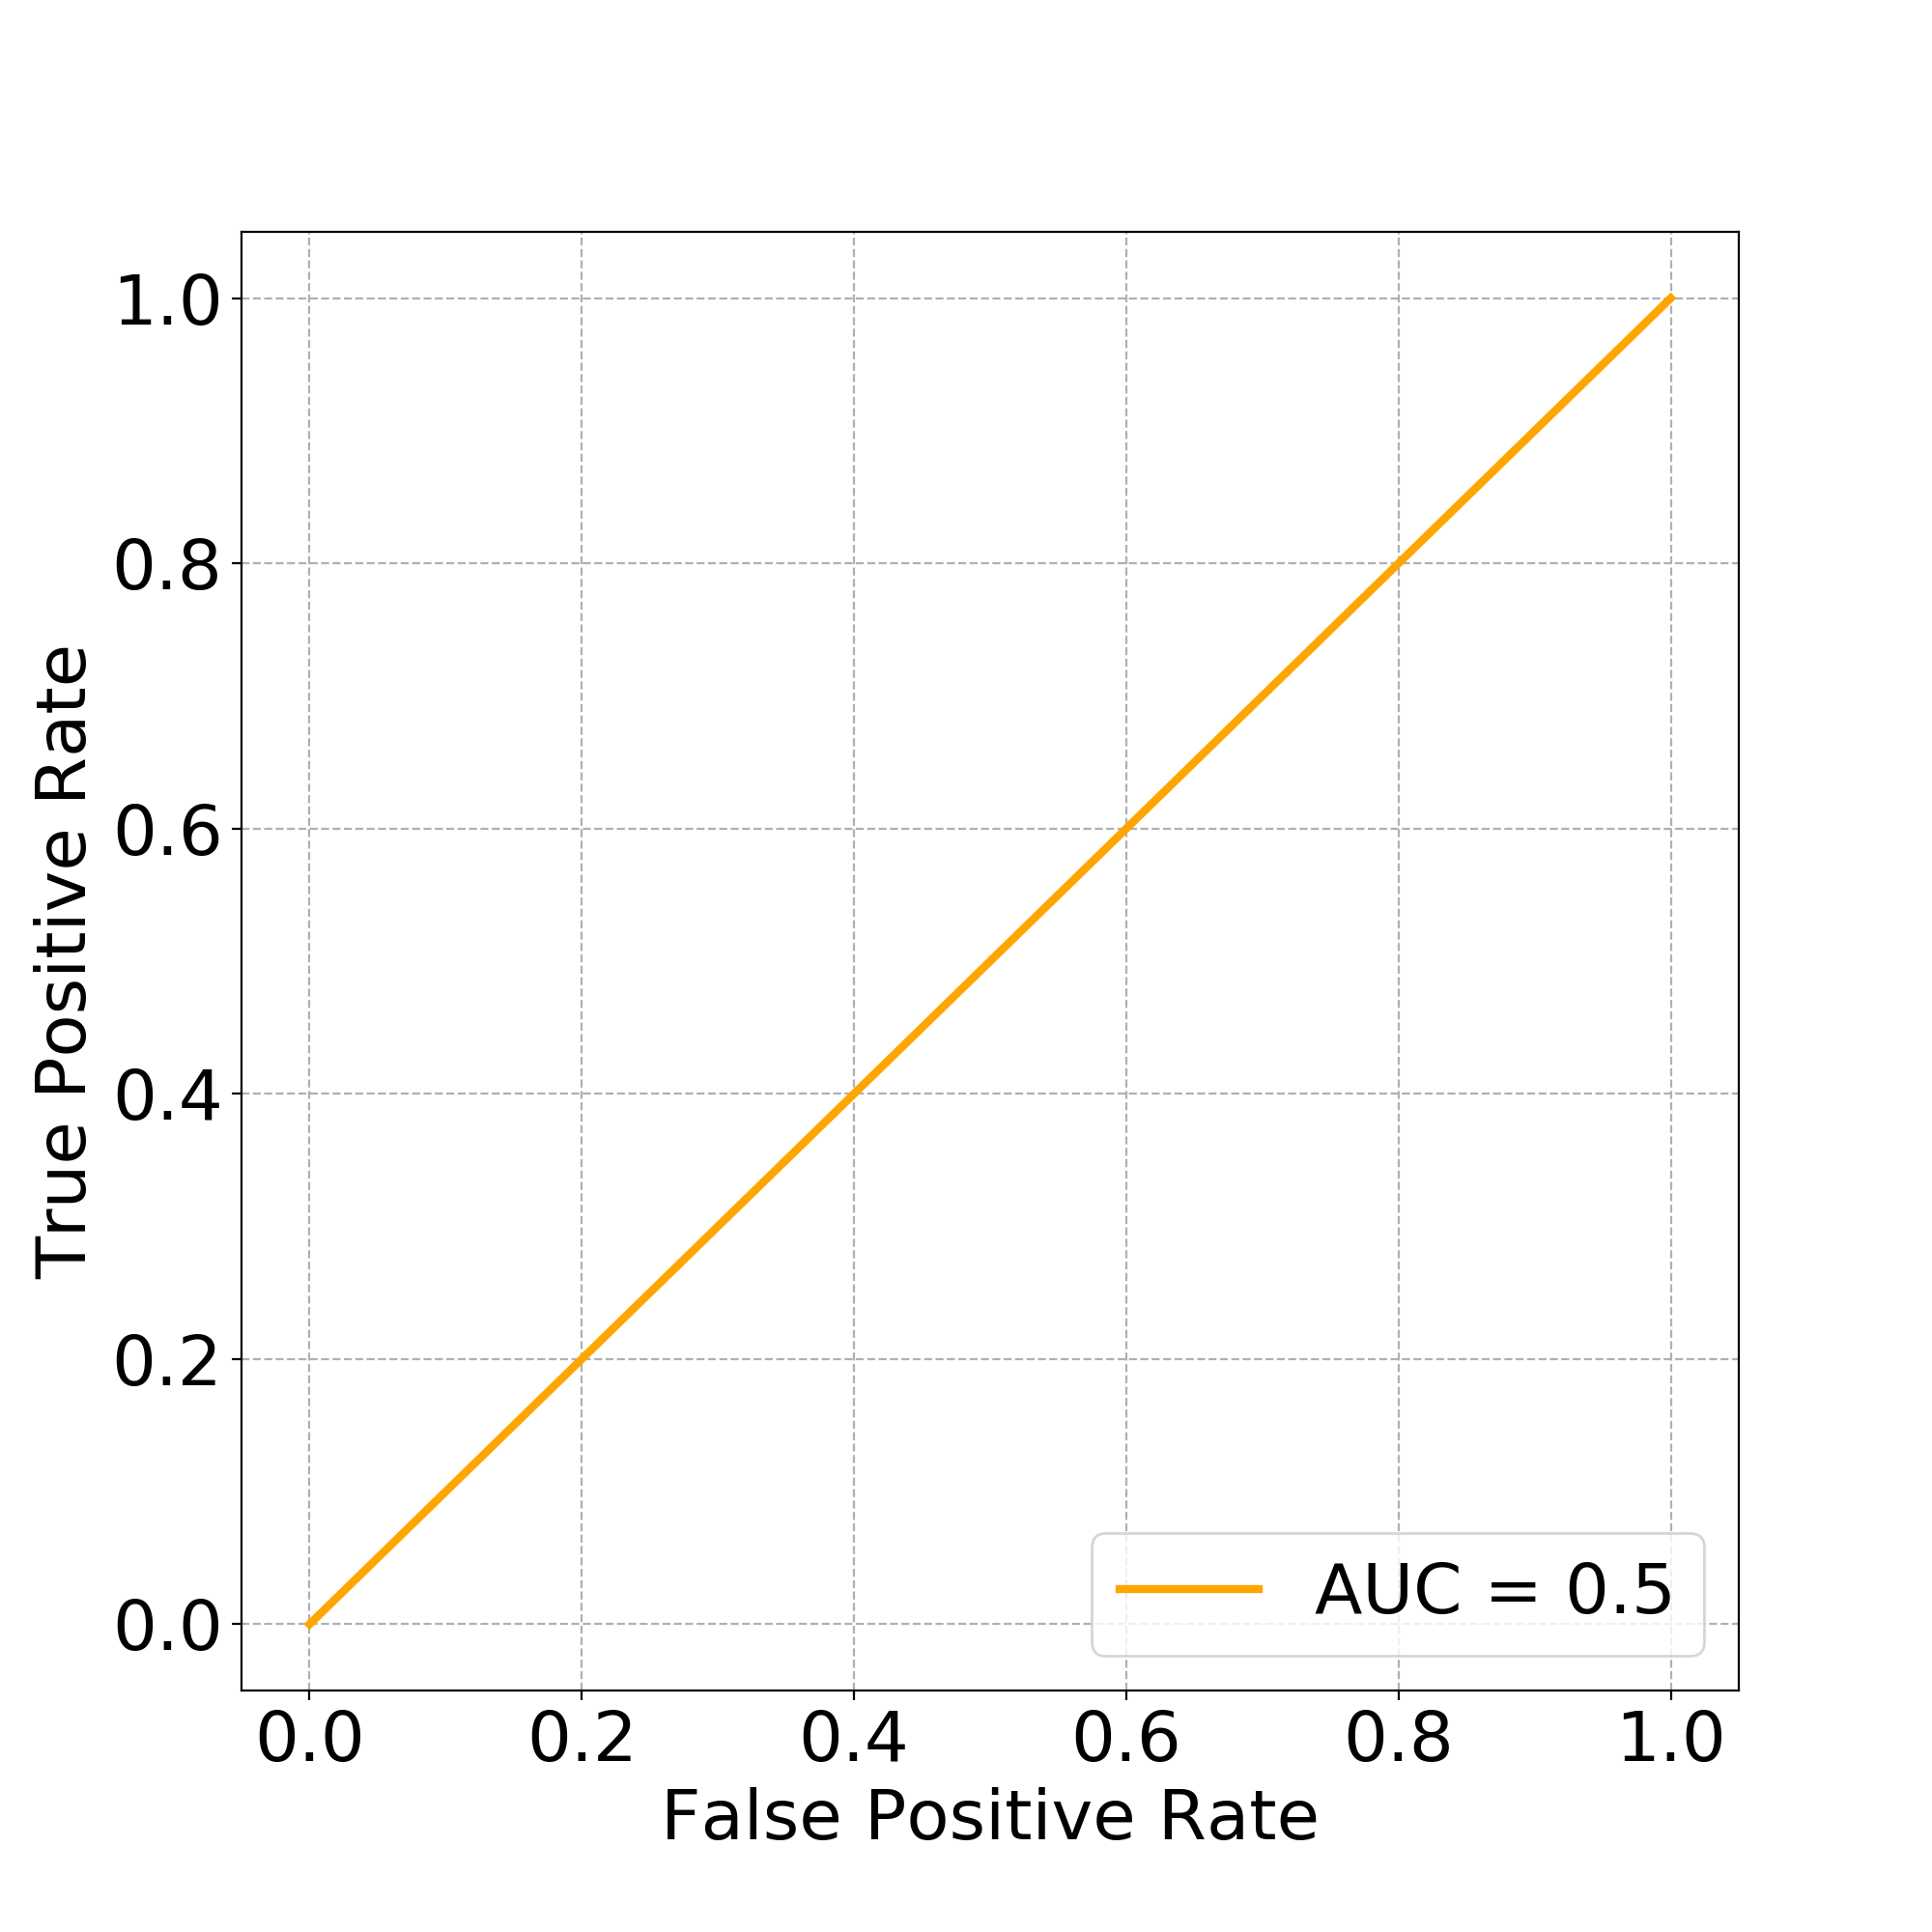
\includegraphics[width=0.45\columnwidth]{roc-3.png}
    \label{fig:roc:3}
  }
  \subfigure[]{
    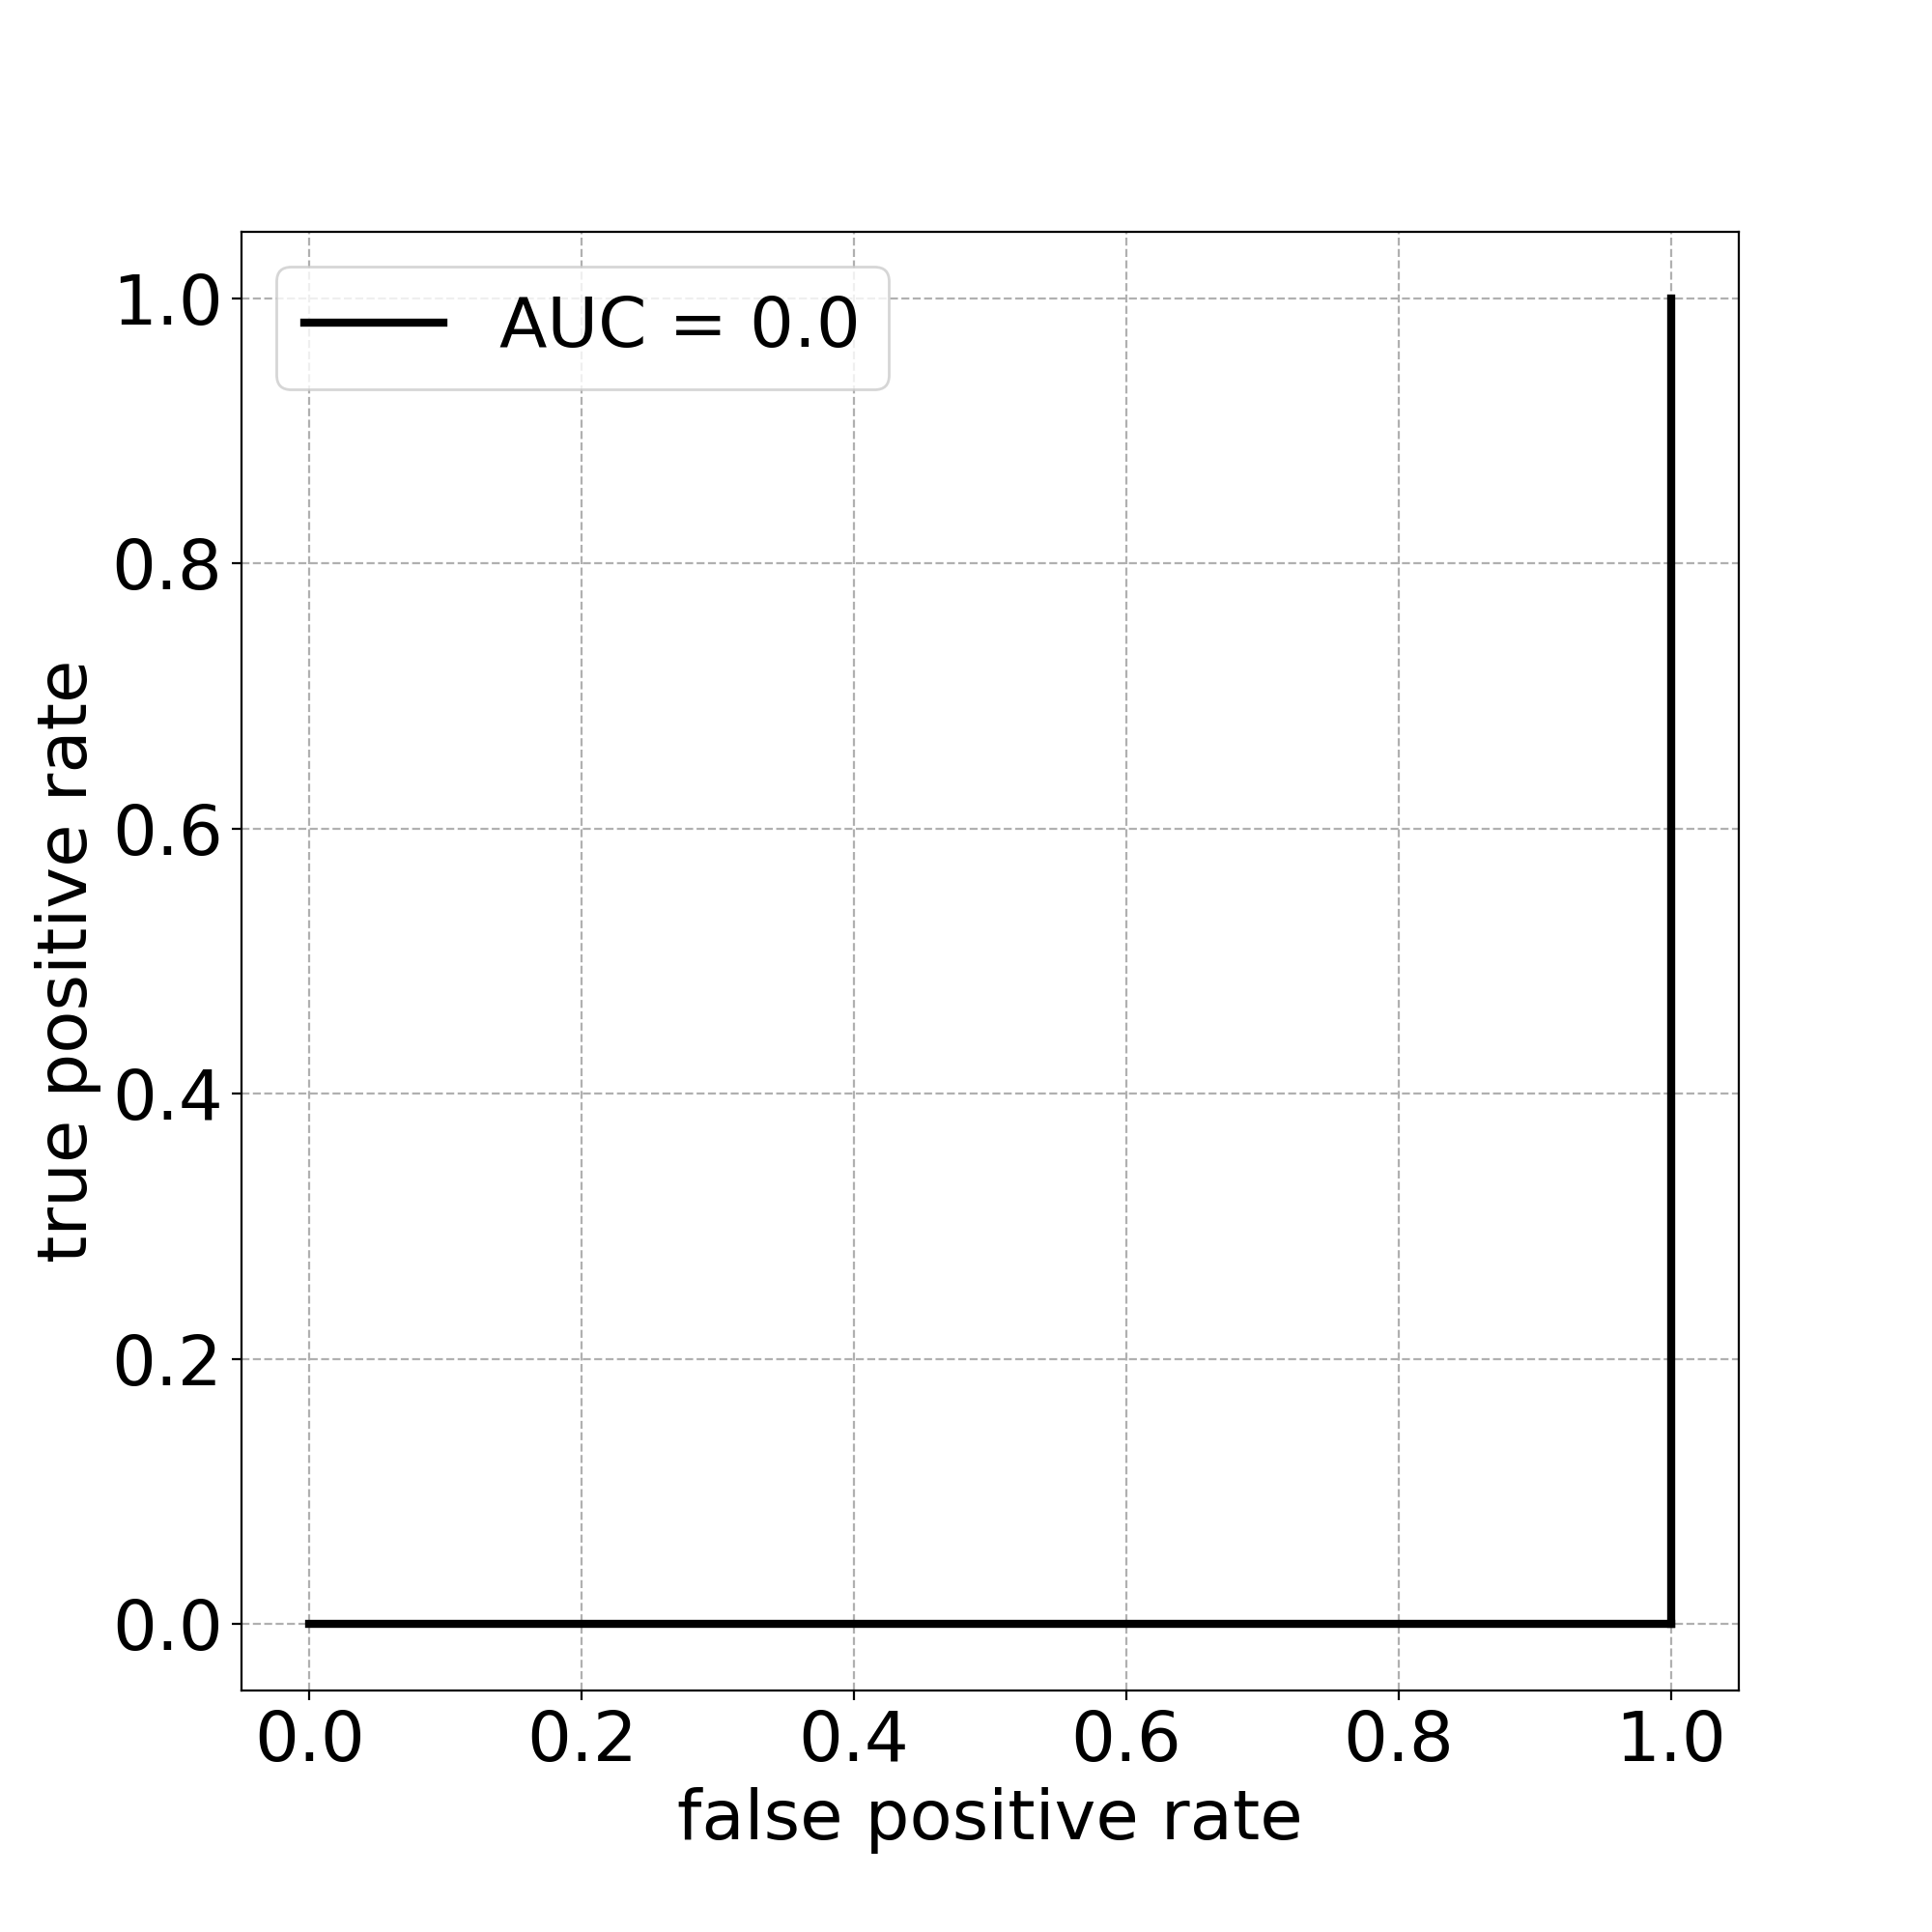
\includegraphics[width=0.45\columnwidth]{roc-4.png}
    \label{fig:roc:3}
  }
  \caption{ตัวอย่างกราฟ ROC Curve แบบต่าง ๆ}
  \label{fig:roc}
\end{figure}
\FloatBarrier

   	\chapter{ผลการทดลอง}
\label{chapter:result}

ในงานวิจัยนี้การทดลองถูกแบ่งออกเป็น 2 ส่วนหลัก ๆ คือ การจัดกลุ่มข้อมูลสองกลุ่ม (Binary Classification) และ การจัดกลุ่มข้อมูลหลายกลุ่ม (Multi-Class Classification) โดยประเภทของข้อมูลที่ถูกใช้ในการทดลองมี 2 ประเภท คือ ข้อมูลแบบมีโครงสร้าง และ ข้อมูลภาพ สำหรับข้อมูลแบบมีโครงสร้างจะมีทั้งหมด 23 ชุดข้อมูล ที่ซึ่งแต่ละชุดข้อมูลจะมีกลุ่มของข้อมูลอยู่ 2 กลุ่ม โดยชุดข้อมูลทั้งหมดนี้จะเป็นชุดข้อมูลที่ไม่สมดุลสำหรับการวัดเปรียบเทียบสมรรถนะเกณฑ์มาตรฐาน (Benchmark) ตามที่ถูกนำเสนอไปใน~\cite{Ding:2011} สำหรับข้อมูลภาพจะมี 2 ชุดข้อมูล คือ CIFAR-100~\cite{Krizhevsky:2009} และ CIFAR-10~\cite{Krizhevsky:2009} โดยทั้งสองนี้เป็นชุดข้อมูลที่สมดุลกันอยู่แล้ว และมีจำนวนกลุ่มข้อมูล 100 และ 10 กลุ่มตามลำดับ แต่จะถูกนำมาดัดแปลงให้ไม่สมดุลเพื่อทำการทดลอง โดยรายละเอียดของการดัดแปลงของ CIFAR-100 และ CIFAR-10 จะถูกอธิบายไว้ในหัวข้อย่อยต่อไป

สำหรับสถาปัตยกรรมของโมเดลที่ใช้ในการทดลองถูกแบ่งออกเป็น 2 ส่วน คือ โมเดลโครงข่ายประสาทเทียมแบบมี 1 Hidden Layer สำหรับการทดลองกับข้อมูลแบบมีโครงสร้าง และ โมเดล ResNet~\citep{He:2016} สำหรับการทดลองกับข้อมูลภาพ

\section{Binary Classification}
\subsubsection{ผลการทดลองกับชุดข้อมูลแบบมีโครงสร้าง}
\subsubsection{ผลการทดลองกับชุดข้อมูล CIFAR-100}
การทดลองใน~\cite{Wang:2016} ได้ทำการดัดแปลง CIFAR-100 โดยการแบ่งชุดข้อมูลออกเป็น 3 ชุดข้อมูลย่อย คือ Tree 1, Tree 2 และ Household และเลือกข้อมูลมา 2 กลุ่มที่แตกต่างกันสำหรับแต่ละชุดข้อมูลย่อย ที่ซึ่งข้อมูลในแต่ละชุดข้อมูลย่อยจะถูกทำให้ไม่สมดุลกัน สำหรับรายละเอียดของกลุ่มข้อมูลในแต่ละชุดข้อมูลย่อยดังนี้

\paragraph{Tree 1}
เป็นชุดข้อมูลที่ประกอบด้วยข้อมูลของกลุ่ม \emph{maple tree} และ \emph{oak tree} โดยจะให้กลุ่ม \emph{maple tree} เป็นกลุ่มข้อมูลส่วนมาก และ \emph{oak tree} เป็นกลุ่มข้อมูลส่วนน้อย

\paragraph{Tree 2}
เป็นชุดข้อมูลที่ประกอบด้วยข้อมูลของกลุ่ม \emph{maple tree} และ \emph{palm tree} โดยจะให้กลุ่ม \emph{maple tree} เป็นกลุ่มข้อมูลส่วนมาก และ \emph{palm tree} เป็นกลุ่มข้อมูลส่วนน้อย

\paragraph{Tree Household}
เป็นชุดข้อมูลที่ประกอบด้วยข้อมูลของกลุ่ม \emph{household furniture} และ \emph{household electrical devices} โดยจะให้กลุ่ม \emph{household furniture} เป็นกลุ่มข้อมูลส่วนมาก และ \emph{household electrical devices} เป็นกลุ่มข้อมูลส่วนน้อย


\label{ex:cifar-100}
\section{Multi-Class Classification}
\subsubsection{ผลการทดลองกับชุดข้อมูล Long-Tailed-Imbalanced CIFAR-10}
ชุดข้อมูล CIFAR-10 จะถูกดัดแปลงให้ไม่สมดุลแบบ Long-Tail
\label{ex:long-tailed-cifar-10}
\subsubsection{ผลการทดลองกับชุดข้อมูล Step-Imbalanced CIFAR-10}
ชุดข้อมูล CIFAR-10 จะถูกดัดแปลงให้ไม่สมดุลแบบ Step
\label{ex:step-cifar-100}
   	\chapter{บทสรุป}
\label{chapter:conclusion}

ในงายวิจัยนี้ ผู้วิจัยได้ศึกษาการทำงานของฟังก์ชันสูญเสียแบบ Mean False Error (MFE) และ Focal Loss (FL) สำหรับการเรียนรู้ของแบบจำลองโครงข่ายประสาทเทียมเชิงลึกอย่างละเอียด เพื่อที่จะหาข้อได้เปรียบของแต่ละฟังก์ชัน ฟังก์ชันสูญเสียทั้งสองดังกล่าวเป็นฟังก์ชันสูญเสียที่ถูกออกแบบมาเพื่อจัดการกับปัญหาความไม่สมดุลกันของข้อมูล
จากผลการศึกษาพบว่าแต่ละฟังก์ชันสูญเสียมีวิธีการจัดการปัญหาความไม่สมดุลกันของข้อมูลที่ต่างกัน และแนวคิดของแต่ละฟังก์ชันสามารถนำมารวมกันได้ เพื่อที่จะใช้ข้อได้เปรียบของทั้งสองฟังก์ชันเพิ่มประสิทธิภาพการเรียนรู้ของโมเดล ด้วยเหตุนี้ผู้วิจัยจึงนำเสนอฟังก์ชันสูญเสียแบบใหม่ที่เรียกว่า Hybrid Loss ที่ซึ่งเป็นการผสมผสานกันระหว่าง MFE และ FL โดยการคำนวณค่าสูญเสียแต่ละตัวอย่างข้อมูลจะคำนวณด้วย FL แต่สำหรับการคำนวณค่าสูญเสียรวมจะนำวิธีการคำนวณค่าสูญเสียรวมของ MFE มาใช้ ผลการทดลองการจัดกลุ่มข้อมูลสองกลุ่มด้วยชุดข้อมูลที่หลากหลายแสดงให้เห็นว่า Hybrid Loss สามารถให้ผลการทดลองในเชิงความแม่นยำที่สูงกว่า MFE และ FL อย่างชัดเจน ซึ่งนั้นหมายความ Hybrid Loss สามารถทำงานได้อย่างดีในการจัดกลุ่มข้อมูลสองกลุ่ม ในอนาคตผู้วิจัยอาจจะทดลอง Hybrid Loss กับการจัดกลุ่มข้อมูลหลายกลุ่ม เพื่อพิสูจน์ว่าแนวคิดของ Hybrid Loss ในตอนนี้สามารถจัดการกับปัญหาความไม่สมดุลกันของข้อมูลหลายกลุ่มได้หรือไม่
    
    \clearpage
    \addcontentsline{toc}{chapter}{บรรณานุกรม}
    \bibliographystyle{IEEEtran}
    \bibliography{reference}
    
    \startappendix
    \chapter{เรื่องที่หนึ่ง}
    
\end{document}